\documentclass[twoside,makeidx]{book}

\usepackage{pdfpages}

% set paper size and margins; needs to be adapted for A5 ideally, we
% should have a document class for conference handbooks where A5
% vs. letter-halved is a class option
\usepackage[
  paperheight=8.5in, 
  paperwidth=5.5in, 
  inner=.75in,
  outer=.5in,
  bottom=.75in,
  top=.75in,
  twoside]{geometry}
\usepackage[T1]{fontenc}
\usepackage{hyperref}
\usepackage[utf8]{inputenc}
\usepackage{textcomp}
\usepackage{graphicx}
\usepackage{color}
\definecolor{mygray}{gray}{0.75}
\usepackage{colortbl}
\usepackage{fancyhdr}
\usepackage[Bjornstrup]{fncychap}
\usepackage{longtable}
\usepackage{tabularx}
\usepackage{lscape}
\usepackage{array}
\usepackage{calc}
\usepackage{csquotes}
\usepackage[american]{babel}
\usepackage{multicol}
\usepackage{multirow}
\usepackage{times}
\usepackage{helvet}
\usepackage[maxnames=25,minnames=3,babel=hyphen]{biblatex}
\usepackage{bibentry}
\usepackage{setspace}
\usepackage{ifthen}
\usepackage{pstricks}
\usepackage{rotating}
\usepackage{makeidx}
\usepackage{marginnote}
\usepackage{ragged2e}

%\providecommand{\BIBand}{and}

\newcommand{\leftheader}{}  
\newcommand{\rightheader}{} 
\pagestyle{fancy}
  % header spec
  %\renewcommand{\headrule}{{\color[rgb]{0.696,0,0}% 
  \renewcommand{\headrule}{{\color[rgb]{0.132,0.125,.46}% 
    \hrule height 2pt width \headwidth}
    \vspace{1pt}%
    {\color{mygray}%
    \hrule height 1pt width \headwidth
  \vspace{-4pt}}}

  \fancyhf{}				       % clear header contents
  %\fancyhead[LE]{\textit{\nouppercase{\leftmark}}}
  %\fancyhead[RO]{\textit{\nouppercase{\rightmark}}} % define header contents
  \fancyhead[LE]{\textit{\nouppercase{\leftheader}}}
  \fancyhead[RO]{\textit{\nouppercase{\rightheader}}} % define header contents

  % footer spec
  \renewcommand{\footrule}{\hrule width \headwidth height 1mm\vskip\footruleskip}
  \renewcommand{\footruleskip}{0.5\normalbaselineskip}
  \fancyfoot[C]{\thepage}			 %define footer conten

%  \rfoot{\setlength{\unitlength}{1mm} % logo in right part of footer
%  \begin{picture}(0,0)
    %\put(-13,-10){\includegraphics[scale=0.3]{images/conf.jpg}}%
%    \put(-10,-5){\includegraphics[scale=0.2]{images/conf.jpg}}%
%  \end{picture}}

\makeatletter
\renewcommand\chapter{\if@openright\cleardoublepage\else\clearpage\fi %let headers/footers show on pages that start a chapter
                    \global\@topnum\z@
                    \@afterindentfalse
                    \secdef\@chapter\@schapter}

\renewcommand{\chaptermark}[1]{\markboth{#1}{}} % show chapter in header w/o numbering
\renewcommand{\sectionmark}[1]{\markright{#1}{}} % show section in headers w/o numbering

% redefine sections to have a horizontal rule and no numbering
\def\section{\@ifstar\unnumberedsection\numberedsection}
\def\numberedsection{\@ifnextchar[%]
  \numberedsectionwithtwoarguments\numberedsectionwithoneargument}
\def\unnumberedsection{\@ifnextchar[%]
  \unnumberedsectionwithtwoarguments\unnumberedsectionwithoneargument}
\def\numberedsectionwithoneargument#1{\numberedsectionwithtwoarguments[#1]{#1}}
\def\unnumberedsectionwithoneargument#1{\unnumberedsectionwithtwoarguments[#1]{#1}}
\def\numberedsectionwithtwoarguments[#1]#2{
  \ifhmode\par\fi
  \removelastskip
  \vskip 3ex\goodbreak
  \refstepcounter{section}%			   % increment counter
  \begingroup
  \noindent\begin{minipage}{\columnwidth}
  \leavevmode\Large\bfseries\raggedright
%  \thesection\  % leave out numbering
  #2 \par\nobreak
  \vskip -.5em
  \noindent\hrulefill\nobreak
  \end{minipage}
  \endgroup
  \vskip 1ex\nobreak
  \markright{#1}{} % add mark to right (secondary) header
  \addcontentsline{toc}{section}{%
%    \protect\numberline{\thesection}% % leave out number
    #1}%
  }
\def\unnumberedsectionwithtwoarguments[#1]#2{
  \ifhmode\par\fi
  \removelastskip
  \vskip 3ex\goodbreak
  \begingroup
  \noindent\begin{minipage}{\columnwidth}
  \leavevmode\Large\bfseries\raggedright
  #2\par\nobreak
  \vskip -.5em
  \noindent\hrulefill\nobreak
  \end{minipage}
  \endgroup
  \vskip 1ex\nobreak
  \markright{#1}{} % add mark to right (secondary) header
  }

% redefine subsections to have a horizontal rule and no numbering
\def\subsection{\@ifstar\unnumberedsubsection\numberedsubsection}
\def\numberedsubsection{\@ifnextchar[%]
  \numberedsubsectionwithtwoarguments\numberedsubsectionwithoneargument}
\def\unnumberedsubsection{\@ifnextchar[%]
  \unnumberedsubsectionwithtwoarguments\unnumberedsubsectionwithoneargument}
\def\numberedsubsectionwithoneargument#1{\numberedsubsectionwithtwoarguments[#1]{#1}}
\def\unnumberedsubsectionwithoneargument#1{\unnumberedsubsectionwithtwoarguments[#1]{#1}}
\def\numberedsubsectionwithtwoarguments[#1]#2{
  \ifhmode\par\fi
  \removelastskip
  \vskip 3ex\goodbreak
  \refstepcounter{subsection}%			   % increment counter
  \begingroup
  \noindent
  \leavevmode\normalsize\bfseries\raggedright
%  \thesubsection\  % leave out numbering
  #2 \par\nobreak
  \endgroup
  \vskip 1ex\nobreak
  \addcontentsline{toc}{subsection}{%
%    \protect\numberline{\thesubsection}% % leave out number
    #1}%
  }
\def\unnumberedsubsectionwithtwoarguments[#1]#2{
  \ifhmode\par\fi
  \removelastskip
  \vskip 3ex\goodbreak
  \begingroup
  \noindent
  \leavevmode\normalsize\bfseries\raggedright
  #2\par\nobreak
  \endgroup
  \vskip 1ex\nobreak
  }

\makeatother

% Clears to an even-numbered page
\def\clearevenpage{
     \clearpage 
     \ifodd\value{page} \hbox{}\newpage\fi
}

% Clears to the back-cover (for logos)
\def\cleartobackcover{
     \clearpage 
     \ifodd\value{page}\pagestyle{empty}\clearevenpage \else\hbox{}\cleardoublepage\pagestyle{empty}\clearevenpage\fi
}

%\renewcommand{\cleardoublepage}{\clearpage}

% Min: index
\makeindex

%\raggedbottom
%\setlength{\parindent}{0pt}
% Unicode issues
% \DeclareUnicodeCharacter{fi}{fi}

% Min: correct column widths
\newlength{\mycolumnwidth}
\setlength{\mycolumnwidth}{\columnwidth}
\addtolength{\mycolumnwidth}{-2ex}

\renewcommand{\textfraction}{.2}
\renewcommand{\bottomfraction}{.8}

\newenvironment{bio}
               {\begin{figure}[b]
                   \centerline{\rule{.5\linewidth}{.5pt}}\vspace{2ex}
                   \setlength{\parskip}{1ex}\setlength{\parindent}{0ex}}
               {\end{figure}}

\setlength{\parindent}{1em}

\fancypagestyle{emptyheader}
{
  \fancyhf{}
  \fancyfoot[C]{\thepage}
}

\newcommand{\setheaders}[2]{%
  \renewcommand{\leftheader}{#1}%
  \renewcommand{\rightheader}{#2}}

\newcommand{\setheadertimezone}[1]{%
  \fancyhead[LO]{\textit{\nouppercase{#1}}}
  \fancyhead[RE]{\textit{\nouppercase{#1}}} % define header contents
}
%%%%%%%%%%%%%%%%%%%%%%%%%%%%%%%%%%%%%%%%%%%%%%%%%%
 
% Macros for the production of Conference Handbooks / Program Brochures from
% ACLPUB bundles from the START conference manager.

\newlength{\w}      % width of the space available for paper entries in a
                    % multi-track schedule
\newlength{\tsl}    % with of a time specification in a schedule
\newlength{\en}     % \en-space
%\newlength{\tmplen}

\setlength{\tabcolsep}{.5ex} 

\newenvironment{SingleTrackSchedule}%
{%
  \settowidth{\en}{--}
  \setlength{\w}{\linewidth}%
  \settowidth{\tsl}{$\,$} % temporary abuse of this length measure
  \addtolength{\w}{-2\tsl}%
  \settowidth{\tsl}{00:00}
  \addtolength{\w}{-2\tsl}%
  \addtolength{\w}{-2\tabcolsep}%
  \addtolength{\w}{-1\en}%
  \begin{longtable}{@{}%
      >{\raggedleft}p{\tsl}%
      @{$\,$}%
      p{1\en}%
      @{$\,$}%
      >{\raggedright}p{\tsl}%
      >{\RaggedRight}p{\w}@{}}%
}{%
  \end{longtable}%
}

\newenvironment{TwoTrackSchedule}{
\settowidth{\en}{--}
\setlength{\w}{\linewidth}%
\settowidth{\tsl}{$\,$}
\addtolength{\w}{-2\tsl}%
\settowidth{\tsl}{\footnotesize 00:00am}
\addtolength{\tsl}{2ex}
\addtolength{\w}{-2\tsl}%
\addtolength{\w}{-2\tabcolsep}%
\addtolength{\w}{-1\en}%
\addtolength{\w}{-1cm}%
\renewcommand{\arraystretch}{1.1}
%\setlength{\tmplen}{\tabcolsep}
%\addtolength{\tmplen}{-.5\arrayrulewidth}
\begin{longtable}{@{}|%
    >{\raggedleft}p{\tsl}%
    @{$\,$}%
    p{1\en}%
    @{$\,$}%
    >{\raggedright}%
    p{\tsl}|%
    >{\centering\arraybackslash}p{.5\w}|%
    >{\centering\arraybackslash}p{.5\w}|@{}}%
}{\end{longtable}}

\newenvironment{ThreeTrackSchedule}{
\settowidth{\en}{--}
\setlength{\w}{\linewidth}%
\settowidth{\tsl}{$\,$}
\addtolength{\w}{-2\tsl}%
\settowidth{\tsl}{00:00am}
\addtolength{\tsl}{2ex}
\addtolength{\w}{-2\tsl}%
\addtolength{\w}{-2\tabcolsep}%
\addtolength{\w}{-1\en}%
\addtolength{\w}{-1cm}%
\renewcommand{\arraystretch}{1.1}
%\setlength{\tmplen}{\tabcolsep}
%\addtolength{\tmplen}{-.5\arrayrulewidth}
\begin{longtable}{@{}%
    >{\raggedleft}p{\tsl}%
    @{$\,$}%
    p{1\en}%
    @{$\,$}%
    >{\raggedright}%
    p{\tsl}|%
    >{\centering\arraybackslash}p{.333\w}|%
    >{\centering\arraybackslash}p{.333\w}|%
    >{\centering\arraybackslash}p{.333\w}@{}}%
}{\end{longtable}}

\newenvironment{FourTrackSchedule}{
\settowidth{\en}{--}
\setlength{\w}{\linewidth}%
\settowidth{\tsl}{$\,$}
\addtolength{\w}{-2\tsl}%
\settowidth{\tsl}{00:00am}
\addtolength{\tsl}{2ex}
\addtolength{\w}{-2\tsl}%
\addtolength{\w}{-2\tabcolsep}%
\addtolength{\w}{-1\en}%
\addtolength{\w}{-1cm}%
\renewcommand{\arraystretch}{1.1}
%\setlength{\tmplen}{\tabcolsep}
%\addtolength{\tmplen}{-.5\arrayrulewidth}
\begin{longtable}{@{}|%
    >{\raggedleft}p{\tsl}%
    @{$\,$}%
    p{1\en}%
    @{$\,$}%
    >{\raggedright}%
    p{\tsl}|%
    >{\centering\arraybackslash}p{.25\w}|%
    >{\centering\arraybackslash}p{.25\w}|%
    >{\centering\arraybackslash}p{.25\w}|%
    >{\centering\arraybackslash}p{.25\w}|@{}}%
}{\end{longtable}}

%%%%%%%%%%% BreakTime Macro %%%%%%%%%%%%%%%%%%%%%%%%%%%%%%%%%%%%%%%%%%%%%%
\newcommand{\BreakTime}[4]{%
% adds a gray background to a break or a break-style event
% #1 start time
% #2 end   time
% #3 number of parallel tracks
% #4 label of the break or break-style event
\multicolumn{3}{c}{\cellcolor[gray]{.8}} & 
\multicolumn{#3}{c}{\cellcolor[gray]{.8}} \\[-3ex]\hline 
\bfseries #1 & -- & \bfseries #2 &
\multicolumn{#3}{c|}{\bfseries #4}}
%%%%%%%%%%%%%%%%%%%%%%%%%%%%%%%%%%%%%%%%%%%%%%%%%%%%%%%%%%%%%%%%%%%%%%%%%%

%%%%%%%%%%% PlenaryEvent Macro %%%%%%%%%%%%%%%%%%%%%%%%%%%%%%%%%%%%%%%%%%%%%%
\newcommand{\PlenaryEvent}[4]{%
% event with nothing else going on in parallel
\bfseries #1 & -- & \bfseries #2 &
\multicolumn{#3}{>{\centering\arraybackslash}p{\w}|@{}}{\bfseries #4}}
%%%%%%%%%%%%%%%%%%%%%%%%%%%%%%%%%%%%%%%%%%%%%%%%%%%%%%%%%%%%%%%%%%%%%%%%%%

%%%%%%%%%%% SessionHeader Macro %%%%%%%%%%%%%%%%%%%%%%%%%%%%%%%%%%%%%%%%%%%%%%
\newcommand{\SingleTrackSessionHeader}[3]{%
% event with nothing else going on in parallel
\ifthenelse{\equal{{#1}}{{}}}{&}{#1 & -- } & #2 
\ifthenelse{\equal{#1}{{}}}{}{\hfill}
&\multicolumn{1}{>{\raggedright\arraybackslash}m{\w}}{\bfseries #3}}
%%%%%%%%%%%%%%%%%%%%%%%%%%%%%%%%%%%%%%%%%%%%%%%%%%%%%%%%%%%%%%%%%%%%%%%%%%

% insert references to the page ranges 
\newcommand{\ppp}[1]{pp. \pageref{#1start}--\pageref{#1end}}

% the following code requires the biblatex package
\DeclareNameFormat{authorswithinitials}{%
  % name format that prints the list of authors with initals
  \ifcase\value{uniquename}%
    \usebibmacro{name:first-last}{\namepartfamily}{\namepartgiveni}{\namepartprefix}{\namepartsuffix}%
    \usebibmacro{name:first-last}{\namepartfamily}{\namepartgiveni}{\namepartprefix}{\namepartsuffix}%
  \or
    \ifuseprefix
      {\usebibmacro{name:first-last}{\namepartfamily}{\namepartgiveni}{\namepartprefix}{\namepartsuffixi}}
      {\usebibmacro{name:first-last}{\namepartfamily}{\namepartgiveni}{\namepartprefixi}{\namepartsuffixi}}%
  \or
    \usebibmacro{name:first-last}{\namepartfamily}{\namepartgiveni}{\namepartprefix}{\namepartsuffix}%
  \fi
  \usebibmacro{name:andothers}}

\DeclareNameFormat{authorlastnames}{%
  % name format that prints the list of author last names
  \ifcase\value{uniquename}%
    \usebibmacro{name:last}{\namepartfamily}{\namepartgiveni}{\namepartprefix}{\namepartsuffix}%
  \or
    \ifuseprefix
      {\usebibmacro{name:last}{\namepartfamily}{\namepartgiveni}{\namepartprefix}{\namepartsuffixi}}
      {\usebibmacro{name:last}{\namepartfamily}{\namepartgiveni}{\namepartprefixi}{\namepartsuffixi}}%
  \or
    \usebibmacro{name:last}{\namepartfamily}{\namepartgiveni}{\namepartprefix}{\namepartsuffix}%
  \fi
  \usebibmacro{name:andothers}}

\DeclareNameFormat{fullauthornames}{%
  % name format that prints the list of authors with full author names
  \ifcase\value{uniquename}%
    \usebibmacro{name:first-last}{\namepartfamily}{\namepartgiven}{\namepartprefix}{\namepartsuffix}%
    \or
    \ifuseprefix
        {\usebibmacro{name:first-last}{\namepartfamily}{\namepartgiven}{\namepartprefix}{\namepartsuffixi}}
        {\usebibmacro{name:first-last}{\namepartfamily}{\namepartgiven}{\namepartprefixi}{\namepartsuffixi}}%
  \or
  \usebibmacro{name:first-last}{\namepartfamily}{\namepartgiven}{\namepartprefix}{\namepartsuffix}%
  \fi
  \usebibmacro{name:andothers}}

% insert the list of authors with first name initials
\DeclareCiteCommand{\citeauthorslastnamesonly}{%
  \boolfalse{citetracker}%
  \boolfalse{pagetracker}%
  \usebibmacro{prenote}%
}{\ifciteindex{\indexnames{labelname}}{}%
  \printnames[authorlastnames]{labelname}%
}{\multicitedelim}{\usebibmacro{postnote}}

% insert the list of authors with first name initials
\DeclareCiteCommand{\citeauthorswithinitials}{%
  \boolfalse{citetracker}%
  \boolfalse{pagetracker}%
  \usebibmacro{prenote}%
}{\ifciteindex{\indexnames{labelname}}{}%
  \printnames[authorswithinitials]{labelname}%
}{\multicitedelim}{\usebibmacro{postnote}}
  
% insert the list of authors with full names
\DeclareCiteCommand{\citefullauthornames}{%
  \boolfalse{citetracker}%
  \boolfalse{pagetracker}%
  \usebibmacro{prenote}%
}{%\ifciteindex{\indexnames{labelname}}{}%
  \indexnames{labelname}%
  \printnames[fullauthornames]{labelname}%
}{\multicitedelim}{\usebibmacro{postnote}}
                     
\DeclareFieldFormat[inproceedings]{citetitle}{#1}

\newcommand{\paperauthor}[1]{{\em #1}}
\newcommand{\papertitle}[1]{\citetitle{#1}}

% insert an entry into a multi-track schedule cell
\newcommand{\paperentry}[1]{%
  \renewcommand{\baselinestretch}{.8}%
  \setlength{\parindent}{0pt}%
    \begin{small}%
      \parbox[t]{\linewidth}{%
        {\em \papertitle{#1}}
        \vspace{.5ex}}\par%
      \vfill
      \parbox[b]{\linewidth}{\raggedright%
        \paperauthor{\citeauthorslastnamesonly{#1}}%
        %% \mbox{}~\dotfill~ {\bfseries p.~\pageref{#1}}
        }%
    \end{small}%
}

\newcommand{\sempaperentry}[1]{%
  &&$\bullet$&
  \parbox[t]{\linewidth}{\raggedright\papertitle{#1}\newline
  {\itshape\paperauthor{\citefullauthornames{#1}}}
\mbox{}~\dotfill~\pageref{#1}}}

\newcommand{\atpaperentry}[2]{%
  \footnotesize\parbox[t]{\linewidth}{\noindent%
    \makebox[0pt][r]{#1\hspace*{\tabcolsep}}{%
      \paperauthor{\citeauthorswithinitials{#2}}}:
    \papertitle{#2}\mbox{}~\dotfill{p.~\pageref{#2}\par}}}

% insert an entry into a poster session index
\newcommand{\posterentry}[1]{%
  \renewcommand{\baselinestretch}{1.2}%
  \settowidth{\w}{\bfseries p.~\pageref{#1}}%
  \addtolength{\w}{1em}%
  \parbox[t]{\linewidth-\w}{\noindent\raggedright{\bfseries\papertitle{#1}}%
    \linebreak[0]\ {---~{\paperauthor{\citeauthorswithinitials{#1}}}}\mbox{}~\dotfill\makebox[0pt][l]%
    {\makebox[\w][r]{\bfseries p.~\pageref{#1}}}\vspace{1em}\par}}

% insert an abstract into a list of abstracts (for posters, no time needed)
\newcommand{\posterabstract}[1]{%
  \noindent%
  \begin{minipage}{\linewidth}%
    \label{#1}%
          {\bfseries\normalsize\papertitle{#1}}\\
          \normalsize\paperauthor{\citefullauthornames{#1}}
  \end{minipage}\vspace{1mm}\\\nopagebreak%
  \noindent{\small\input{auto/abstracts/#1}}\par}

% insert an abstract into a list of abstracts
\newcommand{\paperabstract}[5]{%
  % #1 day
  % #2 time
  % #3 session title
  % #4 location
  % #5 paper id
  \noindent%
  \begin{minipage}{\linewidth}%
    \label{#5}%
      %\rule{\linewidth}{1pt}\linebreak
          {\bfseries\normalsize\papertitle{#5}} \\
          \hfill\normalsize\paperauthor{\citefullauthornames{#5}}
%      {\small #1 #2 --- #4}\vspace{.5ex}\\
          \hfill {\small #2}
%    \parbox[t]{.8\linewidth}{\centering
%      {\bfseries\papertitle{\citetitle{#5}}}\linebreak
%      \paperauthor{\citefullauthornames{#5}}}%
%    \parbox[t]{.2\linewidth}{\raggedleft\small%
%      #1\linebreak #2\linebreak #4}\par\nopagebreak
  %% \begin{center}\label{#5}%
  %%   \sloppy\hyphenpenalty=0%
  %%   %{\small --- Session: #3 --- \vspace{.5em}}\linebreak		% Redundant info? - B
  %%   {\bfseries \citetitle{#5}} \vspace{.5em}\linebreak
  %%   {\itshape    \citefullauthornames{#5}}%\vspace{.5em}\linebreak	% Reduce space between header and abstract - B
  %%   %#1 #2 --- #4\linebreak 						% Redundant info? - B
  \end{minipage}\vspace{1mm}\\\nopagebreak%
  \noindent{\small\input{auto/abstracts/#5}}\par}

\newcommand{\TutorialCoverPage}[4]{%
\vspace*{.25in}
% #1 Tutorial Number
% #2 Tutorial Title
% #3 Tutorial Presenter
% #4 Tutorial Presenter Information
%\begin{minipage}{\linewidth}
\begin{centering}
\includegraphics[height=7.5cm,clip=true]{content/fmatter/conference-logo.eps}\\

\vspace{.5cm}

{\Large
The 2012 Conference of the \linebreak
North American Chapter of the \linebreak
Association for Computational Linguistics: \linebreak
Human Language Technologies}\par

\vspace{3cm}

%\begin{tabular}{@{}>{\centering\arraybackslash}p{.7\linewidth}@{}}
\centerline{\huge\bfseries Tutorial~#1\vspace{.25em}}
{\Large Tutorial Notes}\\

\vspace{1cm}

\begin{minipage}{.7\linewidth}
\centering\Large%\setstretch{1.1}
{\bfseries#2}
\end{minipage}

\vfill

{\itshape\Large #3}\\[.5em]
{#4}\\
\vspace{1cm}

{June 3, 2012}\\
{Montr\'{e}al, Queb\'{e}c, Canada}\\\end{centering}
%\end{minipage}
\clearpage}

\newcommand{\STARSEM}{$^\ast$SEM}

\newcommand{\nix}{\cellcolor{mygray}}
% used for the room occupation tables in the local information section

\newcommand{\mrup}[2]{\multirow{#1}{*}{%
%\rotatebox[origin=c]{90}{#2}}%
\begin{sideways}#2\end{sideways}%
}}

\newcommand{\PaperInSchedule}[4][false]{%
  % #1 (optional) with or without a \pageref to the abstract
  % #2 start time (can be empty)
  % #3 end time (can be empty)
  % #4 paper id
  \ifthenelse{\equal{{#2}}{{}}}{&&\hfill}{#2&--&} % ... start time
  \ifthenelse{\equal{{#3}}{{}}}{$\bullet$}{#3}    %   ... end time
    & \parbox[t]{\linewidth}{\raggedright\papertitle{#4}\newline
      {\paperauthor{\citefullauthornames{#4}}}%
      \ifthenelse{\equal{#1}{true}}{\mbox()~\dotfill~\pageref{#4}}}}

\newcommand{\ScheduleItem}[4][false]{%
  % #1 (optional) with or without a \pageref to the abstract
  % #2 start time (can be empty)
  % #3 end time (can be empty)
  % #4 paper id
  \ifthenelse{\equal{{#2}}{{}}}{&&\hfill}{#2&--&} % ... start time
  \ifthenelse{\equal{{#3}}{{}}}{$\bullet$}{#3}    %   ... end time
    & \parbox[t]{\linewidth}{\raggedright\papertitle{#4}\newline
      {\paperauthor{\citefullauthornames{#4}}}%
      \ifthenelse{\equal{#1}{true}}{\mbox()~\dotfill~\pageref{#4}}}}

\newenvironment{singledaywsprogram}[5]{%
% #1 worshop id
% #2 workshop number
% #3 workshop title
% #4 workshop day
% #5 workshop venue
\section{\textbf{W~#2:} #3}\label{#1}

\begin{center}
{\bfseries\Large #4}\vspace{1em}\par
{\itshape Venue:} #5\vspace{0.75em}\par
{\large\bfseries Program\vspace{0.75em}}\par
\setlength{\w}{\linewidth}
\begin{SingleTrackSchedule}}%
{\end{SingleTrackSchedule}\end{center}}

%% WORKSHOP SCHEDULE %%%%%%%%%%%%%%%%%%%%%%%%%%%%%%%%%%%%%%%%%%%%

%\newlength{\wsscheduleindentation}
%\newlength{\wsschedulelabelwidth}
\newenvironment{wsschedule}[5]{%
  % #1 workshop title
  % #2 workshop number
  % #3 workshop label
  % #4 workshop paper ID
  % #5 workshop location
  %\addcontentsline{toc}{section}{{{\bfseries W~#2:} #4}}

  %\addcontentsline{toc}{section}{{{\bfseries W~#2:} 
  %    \ifthenelse{\equal{#1}{none}}{#4}{#1}}}

  % For workshops numbered 0, don't prepend W0 on the contents page
  \clearpage
  \ifthenelse{\equal{#2}{0}}
%%             {\section{\textbf{#1}}}
             {\section{#1}}
%%
%% For ACL 2017, we do not show the Wx prefix and instead only show the title
%%             {\section[{\bfseries W#2:} #1]{{\bfseries Workshop #2:} #1}}
             {\section{#1}}
             %% {{\addcontentsline{toc}{section}{{#1}}}}
             %% {{\addcontentsline{toc}{section}{{{\bfseries W#2:} #1}}}}

  \markboth{}{}
  \label{#3}
  \begin{center}
%    {\huge{\Large Workshop #2:}\vspace{.5ex}\\
    %% {\Large
    %%   \ifthenelse{\equal{#2}{0}}{{}}{{\huge{Workshop #2:\\\vspace{.5ex}}}}
    %%   #1\par}
    {\ifthenelse{\equal{#4}{0}}{{}}{{Organizers: \paperauthor{\citefullauthornames{#4}}}\par}}
    {\large Venue: #5 \vspace{1em}}\\
    %% {\huge Workshop Program\vspace{1ex}}
  \end{center}
  \markright{{\bfseries W~#2:} #1}{}%
  \begin{list}{{}}{%
      \settowidth{\labelwidth}{\bfseries 12:00pm--12:00pm}
      \setlength{\labelsep}{1ex}
      \setlength{\topsep}{0pt}
      \setlength{\parsep}{0pt}
      \setlength{\listparindent}{0pt}
      \setlength{\itemsep}{.5ex}
      \setlength{\rightmargin}{0pt}
      \setlength{\leftmargin}{\labelwidth}
      \addtolength{\leftmargin}{\labelsep}}
}{\end{list}}

\newcounter{WorkshopCounter}

\newenvironment{tutorial}[4]{%
  \stepcounter{TutorialCounter}
  % #1 short title
  % #2 tutorial bibtex ID
  % #3 date and time
  % #4 location

  % Cannot get \papertitle to expand
  \section[\textbf{T\theTutorialCounter:} {#1}]{Tutorial \theTutorialCounter}
  \begin{center}
    \begin{Large}
      \bfseries \papertitle{#2}\\ \vspace{2em}\par
    \end{Large}
    {\itshape \tutorialauthors{#2}}\vspace{1em}\par
    #3 \vspace{1em}\\
    #4
  \end{center}}

\newcounter{TutorialCounter}

\newcommand{\tutorialauthors}[1]{
    \paperauthor{\citefullauthornames{#1}}}

\newcommand{\wspaperentry}[1]{
  \parbox[t]{\linewidth}{\raggedright\papertitle{#1}\newline
    \paperauthor{\citefullauthornames{#1}}}}

\newcommand{\sessionchair}[2]{
  \emph{Chair: #1 #2}\par\index{#2, #1}}

\newcommand{\papertitleandauthor}[1]{
  {\bfseries \papertitle{#1}}\\
  \paperauthor{\citefullauthornames{#1}}}

\newcommand{\papertableentry}[1]{
  {\scriptsize\papertitle{#1}}\newline
  {\tiny\paperauthor{\citeauthorslastnamesonly{#1}}}}

\newenvironment{SessionOverview}[8]{
  \section[#1]{#1 Overview -- #2}
  \setheaders{#1}{#2}
  \begin{center}
    \righthyphenmin2
    \sloppy
    \begin{tabular}{>{\RaggedRight}p{0.69in}|>{\RaggedRight}p{0.69in}|>{\RaggedRight}p{0.69in}|>{\RaggedRight}p{0.69in}|>{\RaggedRight}p{0.69in}|>{\RaggedRight}p{0.69in}}
      \bf Track A & \bf Track B & \bf Track C & \bf Track D & \bf Track E & \bf Track F \\
      \it #3 & \it #4 & \it #5 & \it #6 & \it #7 & \it #8 \\
      \TrackALoc & \TrackBLoc & \TrackCLoc & \TrackDLoc & \TrackELoc & \TrackFLoc \\
      \hline\hline}
{\end{tabular}\end{center}}

\newenvironment{ThreeSessionOverview}[5]{
  \section[#1]{#1 Overview -- #2}
  \setheaders{#1}{#2}
  \begin{center}
    \righthyphenmin2
    \sloppy
    \begin{tabular}{|>{\RaggedRight}p{1.3in}|>{\RaggedRight}p{1.3in}|>{\RaggedRight}p{1.3in}|}
      \hline
      \bf Track A & \bf Track B & \bf Track C \\\hline
      \it #3 & \it #4 & \it #5 \\
      \TrackALoc & \TrackBLoc & \TrackCLoc \\
      \hline\hline}
{\hline\end{tabular}\end{center}}

\newcommand{\daydate}{DAY, DATE}
\newcommand{\daydateyear}{DAY, DATE, YEAR}
\newcommand{\setdaydateyear}[3]{
  \renewcommand{\daydateyear}{#1, #2, #3\xspace}
  \renewcommand{\daydate}{#1, #2\xspace}}
    
%% defines macros for event venues

% 2015 NAACL Venues

\newcommand{\TrackALoc}{\mbox{TrackALoc}}
\newcommand{\TrackBLoc}{\mbox{TrackBLoc}}
\newcommand{\TrackCLoc}{\mbox{TrackCLoc}}
\newcommand{\TrackDLoc}{\mbox{TrackDLoc}}
\newcommand{\TrackELoc}{\mbox{TrackELoc}}
\newcommand{\TrackFLoc}{\mbox{TrackFLoc}}
\newcommand{\TrackGLoc}{\mbox{TrackGLoc}}
\newcommand{\TrackHLoc}{\mbox{TrackHLoc}}
\newcommand{\TrackILoc}{\mbox{TrackILoc}}

\newcommand{\ShortLoc}{\mbox{}}

\newcommand{\OpeningLoc}{\mbox{OpeningLoc}}
\newcommand{\PresidentialLoc}{\mbox{PresidentialLoc}}
\newcommand{\KeynoteLoc}{\mbox{KeynoteLoc}}
\newcommand{\DistinguishedLoc}{\mbox{DistinguishedLoc}}
\newcommand{\ReviewingLoc}{\mbox{ReviewingLoc}}
\newcommand{\BestLoc}{\mbox{BestLoc}}
\newcommand{\FutureLoc}{\mbox{FutureLoc}}

\newcommand{\BreakfastLoc}{\mbox{}}
\newcommand{\RegistrationLoc}{\mbox{Level 2 Foyer}}


\newcommand{\CoffeeLoc}{\mbox{Level 2 Foyer and Melbourne Room}}
\newcommand{\CoffeeLocTut}{\mbox{Level 2 Foyer}}

\newcommand{\UnknownLoc}{TBD}

\newcommand{\PlenaryLoc}{\mbox{Plenary}}
\newcommand{\PosterSessionLoc}{\mbox{Melbourne Room 1 \& 2}}
\newcommand{\BusinessMeetingLoc}{\mbox{Plenary}}

\newcommand{\PosterLoc}{\PosterSessionLoc}
\newcommand{\DemoLoc}{\PosterSessionLoc}
\newcommand{\LunchLoc}{\PosterSessionLoc}
\newcommand{\StudentLunchLoc}{Showtime Events Centre and Common Man Lawn}

\newcommand{\SocialLoc}{\mbox{Melbourne Sealife Aquarium}}
\newcommand{\BusinessLoc}{\BusinessMeetingLoc}    % business meeting

\newcommand{\InvitedLoc}{\PlenaryLoc}
%\newcommand{\BestLoc}{\PlenaryLoc}
\newcommand{\WelcomeLoc}{\PlenaryLoc}
\newcommand{\WelcomeReceptionLoc}{\mbox{Melbourne Room 1}}

\newcommand{\AclLoc}{\BusinessLoc}
\newcommand{\LifetimeLoc}{\PlenaryLoc}
\newcommand{\ClosingLoc}{\PlenaryLoc}

% Tutorials
\newcommand{\TutLocA}{\mbox{T1 Loc}}
\newcommand{\TutLocB}{\mbox{T2 Loc}}
\newcommand{\TutLocC}{\mbox{T3 Loc}}
\newcommand{\TutLocD}{\mbox{T4 Loc}}
\newcommand{\TutLocE}{\mbox{T5 Loc}}
\newcommand{\TutLocF}{\mbox{T6 Loc}}
\newcommand{\TutLocG}{\mbox{T7 Loc}}
\newcommand{\TutLocH}{\mbox{T8 Loc}}
    
% Workshop locations
\newcommand{\WShopLocA}{\mbox{W1 Loc}}
\newcommand{\WShopLocB}{\mbox{W2 Loc}}
\newcommand{\WShopLocC}{\mbox{W3 Loc}}
\newcommand{\WShopLocD}{\mbox{W4 Loc}}
\newcommand{\WShopLocE}{\mbox{W5 Loc}}
\newcommand{\WShopLocF}{\mbox{W6 Loc}}
\newcommand{\WShopLocG}{\mbox{W7 Loc}}
\newcommand{\WShopLocH}{\mbox{W8 Loc}}
\newcommand{\WShopLocI}{\mbox{W9 Loc}}
\newcommand{\WShopLocJ}{\mbox{W10 Loc}}
\newcommand{\WShopLocK}{\mbox{W11 Loc}}
\newcommand{\WShopLocL}{\mbox{W12 Loc}}
\newcommand{\WShopLocM}{\mbox{W13 Loc}}
\newcommand{\WShopLocN}{\mbox{W14 Loc}}
\newcommand{\WShopLocO}{\mbox{W15 Loc}}
\newcommand{\WShopLocP}{\mbox{W16 Loc}}
\newcommand{\WShopLocQ}{\mbox{W17 Loc}}
\newcommand{\WShopLocR}{\mbox{W18 Loc}}
\newcommand{\WShopLocS}{\mbox{W19 Loc}}




    % macros for event locations
% define macros for session titles here
\newcommand{\DDP}{Discourse, Dialog\linebreak[0] and Pragmatics}
\newcommand{\MT}{Machine\linebreak[0] Translation}
\newcommand{\IE}{Information\linebreak[0] Extraction}
\newcommand{\SLP}{Spoken Language\linebreak[0] Processing}
\newcommand{\ML}{Machine\linebreak[0] Learning}
\newcommand{\LRE}{Language Resources\linebreak[0] and Evaluation}
\newcommand{\PM}{Phonology and Morphology}
\newcommand{\SM}{Semantics}
\newcommand{\SP}{Syntax and Parsing}
\newcommand{\DC}{Discourse}
\newcommand{\CTM}{Document Categorization\linebreak[0] and Topic Modeling}
\newcommand{\SU}{Summarization}
\newcommand{\SSM}{Sentiment and\linebreak[0] Social Media}
%
\newcommand{\MonBEtitle}{\DDP~I}
\newcommand{\MonBWtitle}{\MT~I}
\newcommand{\MonBDtitle}{\IE~I}
%
\newcommand{\MonCEtitle}{\SLP}
\newcommand{\MonCWtitle}{\ML~I}
\newcommand{\MonCDtitle}{\LRE}

\newcommand{\MonBEloc}{\EBR}
\newcommand{\MonBWloc}{\WBR}
\newcommand{\MonBDloc}{\DBR}
\newcommand{\MonCEloc}{\EBR}
\newcommand{\MonCWloc}{\WBR}
\newcommand{\MonCDloc}{\DBR}

\newcommand{\TueDtitle}{Best Paper Awards}
\newcommand{\TueDloc}{\WCBR}

\newcommand{\TueEEtitle}{\PM}
\newcommand{\TueEEloc}{\EBR}
\newcommand{\TueECtitle}{\MT~II}
\newcommand{\TueECloc}{\CBR}
\newcommand{\TueEWtitle}{\SM~I}
\newcommand{\TueEWloc}{\WBR}
\newcommand{\TueEDtitle}{\SP}
\newcommand{\TueEDloc}{\DBR}

\newcommand{\TueFEtitle}{Short papers:\linebreak[0] \DC}
\newcommand{\TueFEloc}{\WBR}
\newcommand{\TueFCtitle}{Short papers:\linebreak[0] \MT}
\newcommand{\TueFCloc}{\CBR}
\newcommand{\TueFWtitle}{Short papers:\linebreak[0] \CTM}
\newcommand{\TueFWloc}{\WBR}
\newcommand{\TueFDtitle}{Short papers:\linebreak[0] Syntax}
\newcommand{\TueFDloc}{\DBR}

\newcommand{\WedGEtitle}{Short Papers: \SSM}
\newcommand{\WedGEloc}{\EBR}
\newcommand{\WedGCtitle}{Short Papers: \SM}
\newcommand{\WedGCloc}{\CBR}
\newcommand{\WedGWtitle}{Short Papers: \SU}
\newcommand{\WedGWloc}{\WBR}

\newcommand{\WedHEtitle}{\SSM}
\newcommand{\WedHEloc}{\EBR}
\newcommand{\WedHCtitle}{\ML~II}
\newcommand{\WedHCloc}{\CBR}
\newcommand{\WedHWtitle}{\DDP~II}
\newcommand{\WedHWloc}{\WBR}

\newcommand{\WedIEtitle}{\SU}
\newcommand{\WedIEloc}{\EBR}
\newcommand{\WedICtitle}{\SM~II}
\newcommand{\WedICloc}{\CBR}
\newcommand{\WedIWtitle}{\CTM~II}
\newcommand{\WedIWloc}{\WBR}
  % session titles and venues

\renewcommand{\normalsize}{\fontsize{8}{9}\selectfont}
\renewcommand{\small}{\fontsize{7}{8}\selectfont}
\renewcommand{\footnotesize}{\fontsize{6}{6}\selectfont}
\renewcommand{\large}{\fontsize{10}{11}\selectfont}
\renewcommand{\Large}{\fontsize{12}{14}\selectfont}
\renewcommand{\huge}{\fontsize{14}{17}\selectfont}

% for each part of the conference, add the .bib file produced with
% meta2bibtex.py here:
\bibliography{auto/ArgMin/papers.bib}
\bibliography{auto/BEA9/papers.bib}
\bibliography{auto/BioNLP/papers.bib}
\bibliography{auto/CLPsych/papers.bib}
\bibliography{auto/CMCL/papers.bib}
\bibliography{auto/CoNLL2014/papers.bib}
\bibliography{auto/ComputEL/papers.bib}
\bibliography{auto/EVENTS/papers.bib}
\bibliography{auto/LLVisInt/papers.bib}
\bibliography{auto/LTCSS/papers.bib}
\bibliography{auto/MORPHFSM/papers.bib}
\bibliography{auto/Metaphor/papers.bib}
\bibliography{auto/NLPSD/papers.bib}
\bibliography{auto/SLPAT2014/papers.bib}
\bibliography{auto/SP14/papers.bib}
\bibliography{auto/WASSA/papers.bib}
\bibliography{auto/WMT14/papers.bib}
\bibliography{auto/conll14st/papers.bib}
\bibliography{auto/demos/papers.bib}
\bibliography{auto/fsnlp/papers.bib}
\bibliography{auto/papers/papers.bib}
\bibliography{auto/shortpapers/papers.bib}
\bibliography{auto/srw/papers.bib}
\bibliography{auto/tacl/papers.bib}
\bibliography{auto/tutorials/papers.bib}

\begin{document}

\fancyfoot[C]{}
%% \input{content/fmatter/cover} 
%% 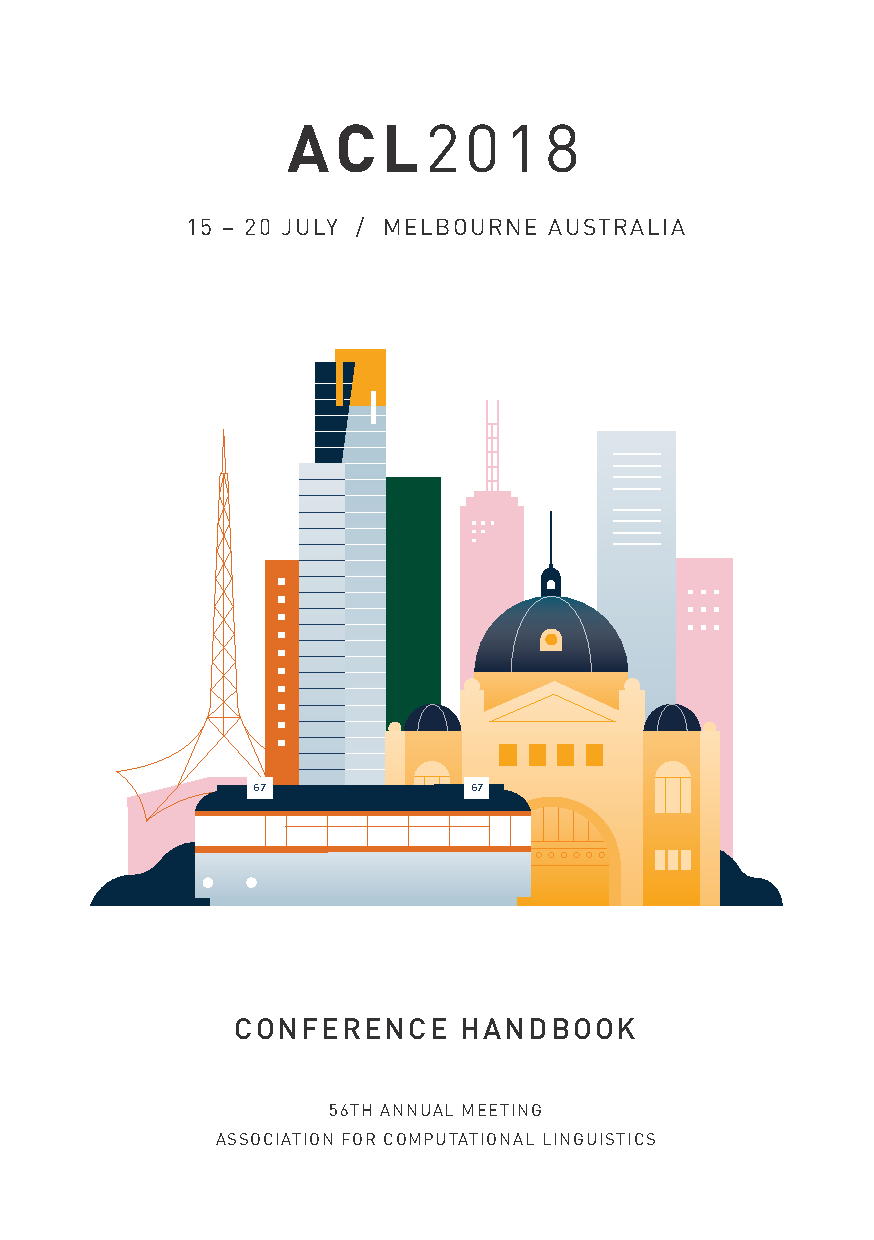
\includepdf[pages={1}]{content/fmatter/cover.pdf}

\fancyfoot[C]{\thepage}

\thispagestyle{empty}
\mbox{}

\vfill
\noindent Handbook production by Matt Post (Johns Hopkins University) \\  
% NAACL HLT 2013 logo by Lucy Roark (VERIFY THIS)
Printing by Omnipress of Madison, Wisconsin
\index{Post, Matt}
\newpage

\frontmatter
%% \input{content/fmatter/splash}\clearpage
\section{Message from the General Chair}\vspace{2em}
\setheaders%
    {Message from the General Chair}%
    {Message from the General Chair}
\thispagestyle{emptyheader}
\begin{large}
\setlength{\parskip}{1ex}

\noindent Welcome to ACL 2014!

I remember with great fondness the first ACL Conference I attended 20 years ago in Las Cruces, New Mexico. Some things have changed: papers presented there that I considered interesting or inconsequential have switched positions in my personal ranking as I learned more and more about our field; single sessions have long been replaced by parallel sessions to accommodate an ever increasing number of research contributions; the number of associated workshops and posters has mushroomed beyond anyone's dream. Almost without noticing, we transitioned from small conferences of a few hundred to conferences that bring together 1000 plus participants from all over the world.  Our field has matured significantly attracting the attention of not only a handful of academics, but successful industries and Research Labs as well.  Some things have stayed the same though: ACL continues to be the pre-eminent conference in our field and the best place to meet and make like-minded friends, discuss tantalizing tricks that you can learn about only in face-to-face communication settings, and celebrate the results we get.

On behalf of the organizing committee, I welcome you to the conference; make the most of it!

\vspace{.2in}
Daniel Marcu \\
\indent General Chair
\end{large}

\index{Marcu, Daniel}

%% \clearpage
%% \section{Message from the Program Committee Co-Chairs}
\setheaders%
    {Message from the Program Committee Co-Chairs}%
    {Message from the Program Committee Co-Chairs}
\thispagestyle{emptyheader}
%\renewcommand{\large}{\fontsize{9}{11}\selectfont}
% that's a hack to make this part nicely fill the pages

\setlength{\parskip}{.7ex}
%\setlength{\parindent}{0pt}

Welcome to the 2015 Conference of the North American Chapter of the
Association for Computational Linguistics -- Human Language
Technologies or NAACL HLT 2015 for short. 

This year, we received the largest number of submissions in the
history of NAACL: a total of 714 submissions with 402 long paper
submissions and 312 short papers submissions. From these, 117 long
papers (62 oral presentations and 55 poster presentations) and 69
short papers (24 oral presentations and 45 poster presentations)
were accepted to appear at the conference.

The submissions to NAACL HLT 2015 were assigned to 18 technical
areas including a new topic area called {\em Language and Vision}.
This track was introduced with an intent to broaden research on
natural language processing that is situated in a rich visual and
perceptual context. We received 16 submissions for this area and
seven of them will be presented at the conference.

For NAACL HLT 2015 we initiated a meta review process, where each
paper received an analysis of the merits of the paper from the area
chair's perspective that was based on the reviewer comments, the
reviewer discussion and the author rebuttal.  We found the meta
reviews very helpful in consolidating the reviews and providing
justifications for final decisions. As this was an experiment this
year, the meta reviews were not sent to the authors.

Based on comments from reviewers, nominations from area chairs, and
rankings from the best paper committee, three papers were selected
to receive the best paper awards at the conference.

Continuing the tradition, NAACL HLT 2015 will feature 19 papers
which were accepted for publication in the Transactions of the
Association for Computational Linguistics (TACL). The TACL papers
were split into 10 oral presentations and 9 poster presentatons.

We are very pleased to have two exciting keynote talks: one by
Professor Lillian Lee (Cornell University) and the other by Professor
Fei-Fei Li (Stanford University).

There are many people to thank for who have worked diligently to
make NAACL HLT 2015 possible. Thanks to the 32 area chairs
for their hard work on recruiting reviewers, managing reviews,
leading discussions, and making recommendations.  All the area
chairs are listed in the Program Committee section of the Front
Matter.  Thanks to Chris Callison-Burch, David Mimno,
Sameer Pradhan, and Philip Resnik for stepping in to serve as area
co-chairs at the last minute when we were faced with an unexpectedly
large number of submissions in some tracks.

Following what was done in the last NAACL conference, we used the
paper assignment tool developed by Mark Dredze to assign papers to
reviewers.  Thanks to Mark Dredze and Jiang Guo for
their hard work on assigning papers to reviewers based on their
preferences.  We had to especially rely on this tool this year
because the distribution of submissions across areas was very
different from past trends.

This program certainly would not be possible without the help of
the 460 reviewers. Their names are listed in the Program Committee
section.  In particular, 116 reviewers from this list were recognized
by the area chairs as best reviewers who have turned in exceptionally
well-written and constructive reviews and who have actively engaged in
the post-rebuttal discussions. The names of the best reviewers are
marked with * in the list of reviewers. 

We are also indebted to the best paper award committee which consists
of Claire Cardie, Daniel Gildea, Daniel Marcu, and Fernando Pereira.
Their time and effort in recommending the best paper awards is much
appreciated.

We also would like to thank Hal Daum\'{e} III, Kristina Toutanova,
and Lucy Vanderwende for generously sharing their experience in
organizing prior NAACL/ACL conferences and for their advice. We are
grateful for the guidance and the support of the NAACL president
Hal Daum\'{e} III, and the NAACL board. We also would like to thank
the publication co-chairs Matt Post and Adam Lopez for putting
together the proceedings and the conference handbook; and Paolo Gai
and Rich Gerber from Softconf for always being responsive to our
requests. 

We would like to thank the ACL Business Manager Priscilla Rasmussen.
She was our {\em go to} person who knew all details of the conference
in and out.  We are very grateful for her help.

Finally, this conference could not have happened without the efforts
of the general chair, Rada Mihalcea. She made sure the various
sections of NAACL organization worked well together. Her monthly
newsletters informed all the organizers about what was being done
by everyone else. We are very thankful for her leadership in the
organization of NAACL HLT 2015.

We hope you will enjoy NAACL HLT 2015!

\noindent
\includegraphics[scale=1.5]{content/fmatter/easteregg.pdf}

\noindent NAACL HLT 2015 Program Co-Chairs \\
Joyce Chai, Michigan State University \\
Anoop Sarkar, Simon Fraser University

\clearpage%{\thispagestyle{emptyheader}\cleardoublepage}
\setheaders{}{}
\markboth{}{} % clear the right header
\markright{}{} % clear the right header

\section{Organizing Committee}{}

\setlength{\parindent}{0pt}

{\bf General Chair} \\
Rada Mihalcea, University of Michigan, USA

{\bf Local Arrangements Chair} \\
Priscilla Rasmussen, ACL Business Manager

{\bf Program Committee Co-chairs} \\
Joyce Chai, Michigan State University, USA \\
Anoop Sarkar, Simon Fraser University, Canada

{\bf Workshop Co-chairs} \\
Cornelia Caragea, University of North Texas, USA \\
Bing Liu, University of Illinois at Chicago, USA

{\bf Tutorial Co-chairs} \\
Yang Liu, University of Texas at Dallas, USA \\
Thamar Solorio, University of Alabama at Birmingham, USA

{\bf Student Research Workshop Co-chairs} \\
\indent \emph{Student Co-chairs} \\
\hspace*{0.2in} Shibamouli Lahiri, University of Michigan, USA \\
\hspace*{0.2in} Karen Mazidi, University of North Texas, USA \\
\hspace*{0.2in} Alisa Zhila, Instituto Politécnico Nacional (National Polytechnic Institute), Mexico \\
\emph{Faculty Advisors} \\
\hspace*{0.2in} Diana Inkpen, University of Ottawa, Canada \\
\hspace*{0.2in} Smaranda Muresan, Columbia University, USA

{\bf Demo Co-chairs} \\
Matt Gerber, University of Virginia, USA \\
Catherine Havasi, Massachusetts Institute of Technology, USA \\
Finley Lacatusu, Language Computer Corporation, USA

{\bf Student Volunteer Coordinator} \\
Annie Louis, University of Edinburgh, UK

{\bf Reviewing Coordinators} \\
Mark Dredze, Johns Hopkins University \\
Jiang Guo, Harbin Institute of Technology

{\bf Local Sponsorship Chair} \\
Kevin B. Cohen, University of Colorado, USA

{\bf Publicity Chair} \\
Saif M. Mohammad, National Research Council Canada

{\bf Publication Co-chairs} \\
Matt Post, John Hopkins University, USA \\
Adam Lopez, University of Edinburgh, UK

{\bf Conference Handbook Editor} \\
Matt Post, Johns Hopkins University

{\bf Website Chair} \\
Peter Ljunglöf, University of Gothenburg and Chalmers University of Technology, Sweden

{\bf Business Manager} \\
Priscilla Rasmussen

%%%%%%%%%%%%%%%%%%%%%%%%%%%%%%%%%%%%%%%%%%%%%%%%%%%%%%%%%%%%%%%%%%%%%%%%

\clearpage
\section{Program Committee}
\setlength{\parindent}{0pt}

\vspace*{0.5cm}

{\bf Program Committee Co-chairs} \\
Joyce Chai, Michigan State University, USA \\
Anoop Sarkar, Simon Fraser University, Canada

{\bf Area Chairs} \\
\emph{Dialogue and Interactive Systems} \\
\hspace*{0.2in} Jason D. Williams, Microsoft Research

\emph{Discourse and Pragmatics} \\
\hspace*{0.2in} Ani Nenkova, University of Pennsylvania \\
\hspace*{0.2in} Vincent Ng, University of Texas at Dallas 

\emph{Generation and Summarization} \\
\hspace*{0.2in} Chris Callison-Burch, University of Pennsylvania \\
\hspace*{0.2in} Fei Liu, Carnegie Mellon University

\emph{Information Extraction and Question Answering} \\
\hspace*{0.2in} Alan Ritter, The Ohio State University \\
\hspace*{0.2in} Bowen Zhou, IBM Research

\emph{Information Retrieval} \\
\hspace*{0.2in} David Smith, Northeastern University

\emph{Language and Vision} \\
\hspace*{0.2in} Julia Hockenmaier, University of Illinois at Urbana-Champaign

\emph{Language Resources and Evaluation} \\
\hspace*{0.2in} Will Lewis, Microsoft Research \\
\hspace*{0.2in} Sameer Pradhan, Harvard University

\emph{Linguistic and Psycholinguistic Aspects of CL} \\
\hspace*{0.2in} William Schuler, The Ohio State University

\emph{Machine Learning for NLP} \\
\hspace*{0.2in} Amarnag Subramanya, Google Research \\
\hspace*{0.2in} Tong Zhang, Baidu Inc. and Rutgers University

\emph{Machine Translation} \\
\hspace*{0.2in} Bill Byrne, Cambridge University \\
\hspace*{0.2in} Hany Hassan, Microsoft Research \\
\hspace*{0.2in} Kevin Knight, Information Sciences Institute, University of Southern California \\
\hspace*{0.2in} Haitao Mi, IBM Research

\emph{NLP for Web, Social Media and Social Sciences} \\
\hspace*{0.2in} Brendan O'Connor, University of Massachusetts \\
\hspace*{0.2in} Philip Resnik, University of Maryland

\emph{NLP-enabled Technology} \\
\hspace*{0.2in} Richard Socher, Stanford University

\emph{Phonology, Morphology, and Word Segmentation} \\
\hspace*{0.2in} Sami Virpioja, Lingsoft and Aalto University

\emph{Semantics} \\
\hspace*{0.2in} Dipanjan Das, Google \\
\hspace*{0.2in} William Dolan, Microsoft Research \\
\hspace*{0.2in} Luke Zettlemoyer, University of Washington

\emph{Sentiment Analysis and Opinion Mining} \\
\hspace*{0.2in} Saif M. Mohammad, National Research Council Canada \\
\hspace*{0.2in} Jerry Zhu, University of Wisconsin-Madison

\emph{Spoken Language Processing} \\
\hspace*{0.2in} Xiaodong He, Microsoft Research

\emph{Tagging, Chunking, Syntax, and Parsing} \\
\hspace*{0.2in} Noah Smith, Carnegie Mellon University \\
\hspace*{0.2in} Yue Zhang, Singapore University of Technology and Design

\emph{Text Categorization and Topic Models} \\
\hspace*{0.2in} Jordan Boyd-Graber, University of Colorado at Boulder \\
\hspace*{0.2in} David Mimno, Cornell University

\clearpage
%
Diamond Sponsors:\\

\begin{tabular}{ c c c }
\raisebox{-0.5\height}{
\includegraphics[width=2cm]{content/sponsors/logos/google.png}} & \raisebox{-0.5\height}{
\includegraphics[width=2cm]{content/sponsors/logos/bytedance-toutiao.png}} & \raisebox{-0.5\height}{
\includegraphics[width=2cm]{content/sponsors/logos/samsung.jpg}} \\ 
\raisebox{-0.5\height}{
\includegraphics[width=2cm]{content/sponsors/logos/Apple_Logo_429C_RGB_090318_clearspace.pdf}} & 
\raisebox{-0.5\height}{
\includegraphics[width=2cm]{content/sponsors/logos/facebook.png}} & 
\end{tabular}
\\

%
\includegraphics[width=3.5cm]{content/sponsors/logos/google.png}\qquad
%
\includegraphics[width=3.5cm]{content/sponsors/logos/bytedance-toutiao.png}\qquad
%
\includegraphics[width=3.5cm]{content/sponsors/logos/samsung.jpg}\\%\qquad
%
\includegraphics[width=3.5cm]{content/sponsors/logos/Apple_Logo_429C_RGB_090318_clearspace.pdf}\qquad
%
\includegraphics[width=3.5cm]{content/sponsors/logos/facebook.png}\\

Platinum Sponsors:\\

\begin{tabular}{ c c c }
	\raisebox{-0.5\height}{
\includegraphics[width=3.2cm]{content/sponsors/logos/amazon.png}} & \raisebox{-0.5\height}{
\includegraphics[width=3.5cm]{content/sponsors/logos/baidu.png}} & \raisebox{-0.5\height}{
\includegraphics[width=3.5cm]{content/sponsors/logos/jingdong.png}} \\ 
	&&\\
	\raisebox{-0.5\height}{
\includegraphics[width=3.5cm]{content/sponsors/logos/rit.png}} & 
	\raisebox{-0.5\height}{
\includegraphics[width=3.5cm]{content/sponsors/logos/tencent.png}} & \\
\end{tabular}
\\
\\
\\

%
\includegraphics[width=3.1cm]{content/sponsors/logos/amazon.png}\qquad
%
\includegraphics[width=3.4cm]{content/sponsors/logos/baidu.png}\qquad
%
\includegraphics[width=3.4cm]{content/sponsors/logos/jingdong.png}\qquad
%
\includegraphics[width=3.4cm]{content/sponsors/logos/rit.png}\qquad
%
\includegraphics[width=3.5cm]{content/sponsors/logos/tencent.png}\\

Gold Sponsors:\\

\begin{tabular}{ c c c }
	\raisebox{-0.5\height}{\LARGE \bf IBM Research} & \raisebox{-0.5\height}{
\includegraphics[width=4cm]{content/sponsors/logos/microsoft.png}} & \raisebox{-0.5\height}{
\includegraphics[width=3.9cm]{content/sponsors/logos/naver.png}} \\
	&&\\
	\raisebox{-0.5\height}{
\includegraphics[width=3.9cm]{content/sponsors/logos/cvte.jpg}} & 
	\raisebox{-0.5\height}{
\includegraphics[width=4.5cm]{content/sponsors/logos/dhcrc.jpg}} & 
\end{tabular}
\\
\\
\\

%IBM Research\qquad 
%
\includegraphics[width=3.6cm]{content/sponsors/logos/microsoft.png}\qquad
%
\includegraphics[width=3.6cm]{content/sponsors/logos/naver.png}\qquad
%
\includegraphics[width=3.6cm]{content/sponsors/logos/cvte.jpg}\\

Silver Sponsors:\\

\begin{tabular}{ c c c c }
	\raisebox{-0.5\height}{
\includegraphics[width=3.5cm]{content/sponsors/logos/nuance.png}}\quad & 
	\raisebox{-0.5\height}{
\includegraphics[width=2.1cm]{content/sponsors/logos/huawei.png}}\quad\quad & 
	\raisebox{-0.5\height}{
\includegraphics[width=2.1cm]{content/sponsors/logos/elsevier.png}}\quad &
	\raisebox{-0.5\height}{
\includegraphics[width=3.5cm]{content/sponsors/logos/duolingo-cropped.jpg}} \\
\end{tabular}


%
\includegraphics[width=3.6cm]{content/sponsors/logos/nuance.png}\qquad\qquad
%
\includegraphics[width=2cm]{content/sponsors/logos/huawei.png}\qquad\qquad
%
\includegraphics[width=2cm]{content/sponsors/logos/elsevier.png}\qquad\qquad
%
\includegraphics[width=3.7cm]{content/sponsors/logos/duolingo.jpg}
%\qquad
%%
\includegraphics[width=3.5cm]{content/sponsors/logos/tencent.png}\\

\newpage

Bronze Sponsors:\\

%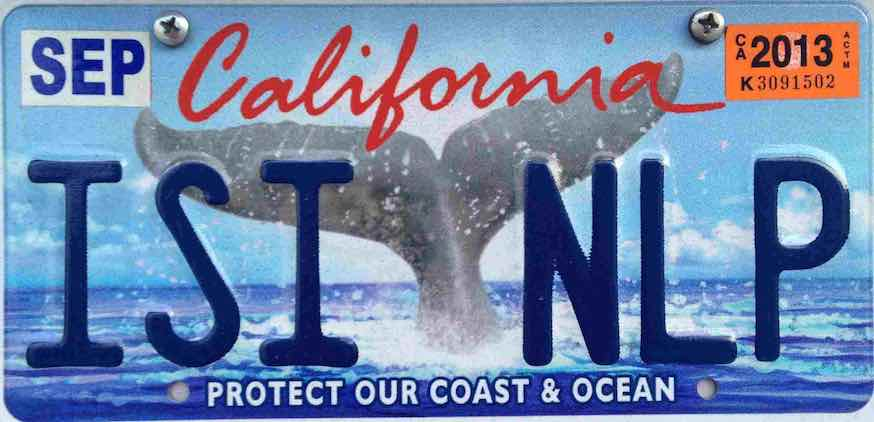
\includegraphics[width=3.6cm]{content/sponsors/logos/isi-nlp.jpg}\qquad 

\begin{tabular}{ c c }
	\raisebox{-0.5\height}{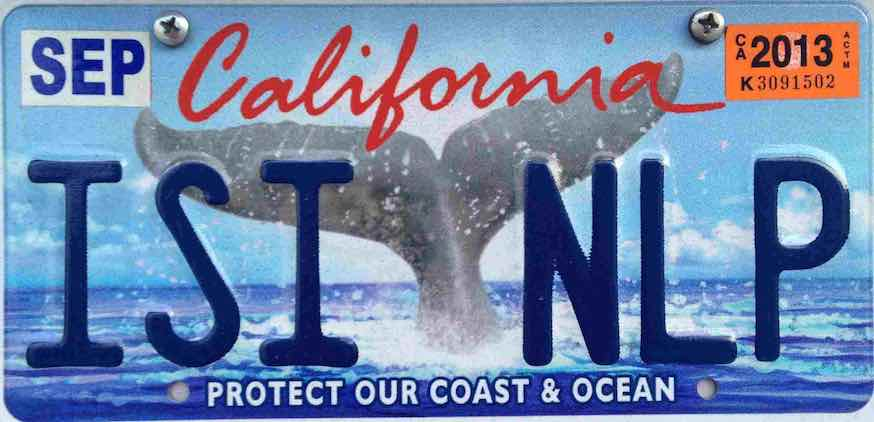
\includegraphics[width=3.5cm]{content/sponsors/logos/isi-nlp.jpg}}\quad\quad & \raisebox{-0.5\height}{
\includegraphics[width=6.5cm]{content/sponsors/logos/dstg.pdf}}\quad\quad \\
\end{tabular}
\\
\\

%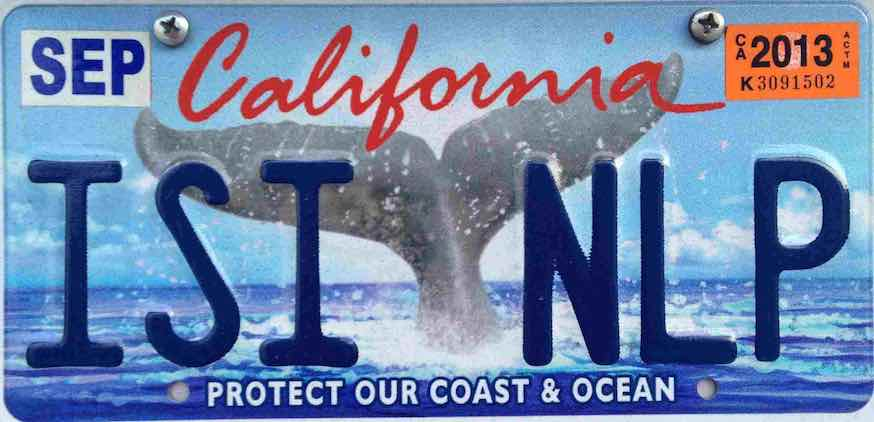
\includegraphics[width=3.6cm]{content/sponsors/logos/isi-nlp.jpg}\qquad 
%\includegraphics[width=3.6cm]{content/sponsors/logos/DSTGroup-Logo-Vert.jpg}

Supporters: \\

\begin{tabular}{ c c }
	\raisebox{-0.5\height}{
\includegraphics[width=3.5cm]{content/sponsors/logos/roam.png}}\quad\quad & \raisebox{-0.5\height}{
\includegraphics[width=3.5cm]{content/sponsors/logos/sap.png}}\quad\quad \\
\end{tabular}
\\
\\

%
\includegraphics[width=3.5cm]{content/sponsors/logos/roam.png} \qquad
%
\includegraphics[width=3.5cm]{content/sponsors/logos/sap.png}\\

Student Volunteers Sponsors: \\

\quad\enskip\includegraphics[width=3.5cm]{content/sponsors/logos/data61.png}

\clearpage%{\thispagestyle{emptyheader}\cleardoublepage}
\setheaders{}{}

\setcounter{tocdepth}{2}
\tableofcontents
\mainmatter
\pagestyle{fancy}

%\input{content/fmatter/local-info}
\clearpage

%% MAIN CONFERENCE %%%%%%%%%%%%%%%%%%%%%%%%%%%%%%%%%%%%%%%%%%%%%%

%% \chapter{Tutorials: Sunday, June 22}
\thispagestyle{emptyheader}
\setheaders{Tutorials}{Sunday, June 22, 2014}
%\addcontentsline{toc}{chapter}{Sunday, Jun 9, 2013: Tutorials}
\setlength{\parindent}{0in}
\setlength{\parskip}{2ex}
\renewcommand{\baselinestretch}{0.87}

\section*{Overview}
\renewcommand{\arraystretch}{1.2}
\begin{SingleTrackSchedule}
  7:30 & -- & 6:00 &
  {\bfseries Registration} \hfill (\UnknownLoc)
  \\
  7:30 & -- & 9:00 &
  {\bfseries Breakfast} \hfill (\UnknownLoc)
  \\
  9:00 & -- & 12:30 &
  {\bfseries Morning Tutorials} \hfill
  \\
  & & & \papertitle{tutorials-001}\hfill (\TutLocA)\newline
  \tutorialauthors{tutorials-001} \\
  \\
  & & & \papertitle{tutorials-002}\hfill (\TutLocB)\newline
  \tutorialauthors{tutorials-002} \\
  \\
  & & & \papertitle{tutorials-003}\hfill (\TutLocC)\newline
  \tutorialauthors{tutorials-003} \\
  \\
  & & & \papertitle{tutorials-004}\hfill (\TutLocD)\newline
  \tutorialauthors{tutorials-004} \\
  \\
  12:30 & -- & 2:00 &
  {\bfseries Lunch break} \hfill (\UnknownLoc)
  \\
  2:00 & -- & 5:30 &
  {\bfseries Afternoon Tutorials} \hfill
  \\
  & & & \papertitle{tutorials-005}\hfill (\TutLocE)\newline
  \tutorialauthors{tutorials-005} \\
  \\
  & & & \papertitle{tutorials-006}\hfill (\TutLocF)\newline
  \tutorialauthors{tutorials-006} \\
  \\
  & & & \papertitle{tutorials-007}\hfill (\TutLocG)\newline
  \tutorialauthors{tutorials-007} \\
  \\
  & & & \papertitle{tutorials-008}\hfill (\TutLocH)\newline
  \tutorialauthors{tutorials-008} \\
  \\
  6:00 & -- & 9:00 &
  {\bfseries Welcome Reception} \hfill (\UnknownLoc)
  \\
  6:50 & -- & 9:30 &
  {\bfseries Poster and Dinner Session I: TACL Papers, Long Papers, Short Papers, Student Research Workshop; Demonstrations} \hfill (\UnknownLoc)
  \\
\end{SingleTrackSchedule}

\clearpage\begin{bio}
  {\bfseries Trevor Cohn} is a Senior Lecturer and ARC Future Fellow at the University of
  Melbourne. His research deals with probabilistic machine learning models, particularly structured
  prediction and non-parametric Bayesian models. He has recently published several seminal papers on
  Gaussian Process models for NLP with applications ranging from translation evaluation to temporal
  dynamics in social media.

  {\bfseries Daniel Preoţiuc-Pietro} is a Research Associate at the University of Sheffield. His
  research involves applying machine learning models to model large volumes of data, usually from
  social media. Applications include forecasting future behaviours of text, users or real world
  quantities (e.g. political voting intention), user geo-location and impact.

  {\bfseries Neil Lawrence} is a Professor at the University of Sheffield. He is one of the foremost
  experts on Gaussian Processes and non-parametric Bayesian inference, with a long history of
  publications and innovations in the field, including their application to multi-output scenarios,
  unsupervised learning, deep networks and scaling to big data. He has been program chair for top
  machine learning conferences (NIPS, AISTATS), and has run several past tutorials on Gaussian
  Processes.

  \index{Cohn, Trevor}
  \index{Preoţiuc-Pietro, Daniel}
  \index{Lawrence, Neil}
\end{bio}

\begin{tutorial}{Gaussian Processes for Natural Language Processing}
  {Trevor Cohn (University of Melbourne), Daniel Preoţiuc-Pietro (University of Sheffield), Neil Lawrence (University of Sheffield)}
  {Sunday, June 22, 2014, 9:00 -- 12:30pm}
  {\TutLocA}

This tutorial aims to cover the basic motivation, ideas and theory of Gaussian Processes and several applications to natural language processing tasks. Gaussian Processes (GPs) are a powerful modelling framework incorporating kernels and Bayesian inference, and are recognised as state-of-the-art for many machine learning tasks. This tutorial will focus primarily on regression and classification, both fundamental techniques of wide-spread use in the NLP community. We argue that the GP framework offers many benefits over commonly used machine learning frameworks, such as linear models (logistic regression, least squares regression) and support vector machines (SVMs). GPs have the advantage of being a fully Bayesian model, giving a posterior over the desired variables. Their probabilistic formulation allows for much wider applicability in larger graphical models, unlike SVMs. Moreover, several properties of Gaussian distributions means that GP (regression) supports analytic formulations for the posterior and predictive inference, avoiding the many approximation errors that plague approximate inference techniques in common use for Bayesian models (e.g. MCMCM, variational Bayes).

GPs provide an elegant, flexible and simple means of probabilistic inference. GPs have been actively researched since the early 2000s, and are now reaching maturity: the fundamental theory and practice is well understood, and now research is focused into their applications, and improve inference algorithms, e.g. for scaling inference to large and high-dimensional datasets. Several open-source packages (e.g. GPy and GPML) have been developed which allow for GPs to be easily used for many applications. This tutorial aims to present the main ideas and theory behind GPs and recent applications to NLP, emphasising their potential for widespread application across many NLP tasks.
\end{tutorial}

\clearpage\begin{bio}
{\bfseries Liang Huang} is an Assistant Professor at the City University of New York (CUNY). He graduated in 2008 from Penn and has worked as a Research Scientist at Google and a Research Assistant Professor at USC/ISI. His work is mainly on the theoretical aspects (algorithms and formalisms) of computational linguistics, as well as theory and algorithms of structured learning. He has received a Best Paper Award at ACL 2008, several best paper nominations (ACL 2007, EMNLP 2008, and ACL 2010), two Google Faculty Research Awards (2010 and 2013), and a University Graduate Teaching Prize at Penn (2005). He has given two tutorials at COLING 2008 and NAACL 2009, being the most popular tutorial at both venues.

{\bfseries Kai Zhao} is a Ph.D. candidate at the City University of New York (CUNY), working with Liang Huang. He received his B.S. from the University of Science and Technology in China (USTC). He has published on structured prediction, online learning, machine translation, and parsing algorithms. He was a summer intern with IBM TJ Watson Research Center in 2013.

{\bfseries Lemao Liu} is a postdoctoral research associate at the City University of New York (CUNY), working with Liang Huang. He received his Ph.D. from the Harbin Institute of Technology in 2013. Much of his Ph.D. work was done while visiting NICT, Japan, under the guidance of Taro Watanabe. His research area is machine translation and machine learning.
\end{bio}

\begin{tutorial}{Scalable Large-Margin Structured Learning: Theory and Algorithms}
  {Liang Huang (CUNY), Kai Zhao (CUNY), and Lemao Liu (CUNY)}
  {Sunday, June 22, 2014, 9:00 -- 12:30pm}
  {\TutLocB}

Much of NLP tries to map structured input (sentences) to some form of
structured output (tag sequences, parse trees, semantic graphs, or
translated/paraphrased/compressed sentences). Thus structured
prediction and its learning algorithm are of central importance to us
NLP researchers. However, when applying machine learning to structured
domains, we often face scalability issues for two reasons:

\begin{enumerate}
\item Even the fastest exact search algorithms for most NLP problems
(such as parsing and translation) is too slow for repeated use on the
training data, but approximate search (such as beam search)
unfortunately breaks down the nice theoretical properties (such as
convergence) of existing machine learning algorithms.

\item Even with inexact search, the scale of the training data in NLP
still makes pure online learning (such as perceptron and MIRA) too
slow on a single CPU.
\end{enumerate}

This tutorial reviews recent advances that address these two
challenges. In particular, we will cover principled machine learning
methods that are designed to work under vastly inexact search, and
parallelization algorithms that speed up learning on multiple CPUs. We
will also extend structured learning to the latent variable setting,
where in many NLP applications such as translation and semantic
parsing the gold-standard derivation is hidden.

\end{tutorial}

\clearpage\begin{bio}
{\bfseries Florian Metze} received his PhD from Universitat Karlsruhe (TH) in 2005. He worked as a Senior Research Scientist at Deutsche Telekom Laboratories (T-Labs) and joined Carnegie Mellon University's faculty in 2009. His interests includes speech and audio processing, and user interfaces.

{\bfseries Koichi Shinoda} received his D.\ Eng. from Tokyo Institute of Technology in 2001. In 1989, he joined NEC Corporation. From 1997 to 1998, he was a visiting scholar with Bell Labs, Lucent Technologies. He is currently a Professor at the Tokyo Institute of Technology. His research interests include speech recognition, video information retrieval, and human interfaces.
\end{bio}

\begin{tutorial}{Semantics for Large-Scale Multimedia: New Challenges for NLP}
  {Florian Metze (CMU) and Koichi Shinoda (TokyoTech)}
  {Sunday, June 22, 2014, 9:00 -- 12:30pm}
  {\TutLocC}

Thousands of videos are constantly being uploaded to the web, creating
a vast resource, and an ever-growing demand for methods to make them
easier to retrieve, search, and index. As it becomes feasible to
extract both low-level as well as high-level (symbolic) audio, speech,
and video features from this data, these need to be processed further,
in order to learn and extract meaningful relations between these. The
language processing community has made huge process in analyzing the
vast amounts of very noisy text data that is available on the
Internet. While it is very difficult to create semantic units of
low-level image descriptors or non-speech sounds by themselves, it is
comparatively easy to ground semantics in the word output of a speech
recognizer, or text data that is loosely associated with a video. This
creates an opportunity for NLP researchers to use their unique skills,
and make significant contributions to solve tasks on data that is even
noisier than web text, but (we argue) even more interesting and
challenging.

This tutorial aims to present to the NLP community the state of the
art in audio and video processing, by discussing the most relevant
tasks at NIST's TREC Video Retrieval Evaluation (TRECVID) workshop
series. We liken "Semantic Indexing" (SIN) task, in which a system
must identify occurrences of concepts such as "desk", or "dancing" in
a video to the word spotting approach. We then proceed to explain more
recent, and challenging tasks, "Multimedia Event Detection" (MED) and
"Multimedia Event Recounting" (MER), which can be compared to
transcription and summarization tasks. Finally, we will present an
easy way to get started in multi-media analysis using Virtual Machines
from the ``Speech Recognition Virtual Kitchen'', which will enable
tutorial participants to perform hands-on experiments during the
tutorial, and at home.

\end{tutorial}

\clearpage\begin{bio}
\small

{\bfseries Dan Roth} is a Professor in the Department of Computer Science at the University of Illinois at Urbana-Champaign and the Beckman Institute of Advanced Science and Technology (UIUC) and a University of Illinois Scholar. He is a fellow of AAAI, ACL and the ACM. Roth has published broadly in machine learning, natural language processing, knowledge representation and reasoning and received several paper, teaching and research awards. He has developed several machine learning based natural language processing systems that are widely used in the computational linguistics community and in industry and has presented invited talks and tutorials in several major conferences. Over the last few years he has worked on Entity Linking and Wikification. He has given several tutorials at ACL/NAACL/ECL and other forums.

{\bfseries Heng Ji} is the Edward G. Hamilton Development Chair Associate Professor in Computer Science Department of Rensselaer Polytechnic Institute. Her research interests focus on Natural Language Processing, especially on Cross-source Information Extraction and Knowledge Base Population. She coordinated the NIST TAC Knowledge Base Population task in 2010, 2011 and 2014 and has published several papers on entity linking and Wikification.

{\bfseries Ming-Wei Chang} is a researcher at Microsoft Research. His research interests are in machine learning and natural language understanding. He currently focuses on using large-scale structured and unstructured data for semantic understanding. Specially, he is interested in developing algorithms for entity linking that are effective for short and noisy text.

{\bfseries Taylor Cassidy} is a Postdoctoral Researcher at U.S. Army Research Laboratory \& IBM Research. His research interests include Cross-lingual Entity Linking and Wikification for social media.
\end{bio}

\begin{tutorial}{Wikification and Beyond: The Challenges of Entity and Concept Grounding}
  {Dan Roth (UIUC), Heng Ji (RPI), Ming-Wei Chang (MSR), Taylor Cassidy (ARL, IBM)}
  {Sunday, June 22, 2014, 9:00 -- 12:30pm}
  {\TutLocD}

Contextual disambiguation and grounding of concepts and entities in natural language text are essential to moving forward in many natural language understanding related tasks and are fundamental to many applications. The Wikification task aims at automatically identifying concept mentions appearing in a text document and linking them to (or “grounding them in”) concept referents in a knowledge base (KB) (e.g., Wikipedia). For example, consider the sentence, "The Times report on Blumenthal (D) has the potential to fundamentally reshape the contest in the Nutmeg State.". A Wikifier should identify the key entities and concepts (Times, Blumental, D and the Nutmeg State), and disambiguate them by mapping them to an encyclopedic resource revealing, for example, that “D” here represents the Democratic Party, and that “the Nutmeg State” refers Connecticut. Wikification may benefit both human end-users and Natural Language Processing (NLP) systems. When a document is Wikified a reader can more easily comprehend it, as information about related topics and relevant enriched knowledge from a KB is readily accessible. From a system-to-system perspective, a Wikified document conveys the meanings of its key concepts and entities by grounding them in an encyclopedic resource or a structurally rich ontology.

The primary goals of this tutorial are to review the framework of Wikification and motivate it as a broad paradigm for cross-source linking for knowledge enrichment. We will present and discuss multiple dimensions of the task definition, present the basic building blocks of a state-of-the-art Wikifier system, share some key lessons learned from the analysis of evaluation results, and discuss recently proposed ideas for advancing work in this area along with some of the key challenges. We will also suggest some research questions brought up by new applications, including interactive Wikification, social media, and censorship. The tutorial will be useful for both senior and junior researchers with interests in cross-source information extraction and linking, knowledge acquisition, and the use of acquired knowledge in natural language processing and information extraction. We will try to provide a concise roadmap of recent perspectives and results, as well as point to some of our Wikification resources that are available to the research communities.

\end{tutorial}

\clearpage\begin{bio}
{\bfseries Phil Blunsom} is an Associate Professor at the University of Oxford's Department of Computer Science. His research centres on the probabilistic modelling of natural languages, with a particular interest in automating the discovery of structure and meaning in text.

{\bfseries Georgiana Dinu} is a postdoctoral researcher at the University of Trento. Her research revolves around distributional semantics with a focus on compositionality within the distributional paradigm.

{\bfseries Edward Grefenstette} is a postdoctoral researcher at Oxford's Department of Computer Science. He works on the relation between vector representations of language meaning and structured logical reasoning. His work in this area was recently recognised by a best paper award at *SEM 2013.

{\bfseries Karl Moritz Hermann} is a final-year DPhil student at the Department of Computer Science in Oxford. His research studies distributed and compositional semantics, with a particular emphasis on mechanisms to reduce task-specific and monolingual syntactic bias in such representations.
\end{bio}

\begin{tutorial}{New Directions in Vector Space Models of Meaning}
  {Phil Blunsom (Oxford), Georgiana Dinu (Trento), Edward Grefenstette (Oxford), and Karl Moritz Hermann (Oxford)}
  {Sunday, June 22, 2014, 2:00 -- 5:30pm}
  {\TutLocE}

Symbolic approaches have dominated NLP as a means to model syntactic and semantic aspects of natural language. While powerful inferential tools exist for such models, they suffer from an inability to capture correlation between words and to provide a continuous model for word, phrase, and document similarity. Distributed representations are one mechanism to overcome these constraints.

This tutorial will supply NLP researchers with the mathematical and conceptual background to make use of vector-based models of meaning in their own research. We will begin by motivating the need for a transition from symbolic representations to distributed ones. We will briefly cover how collocational (distributional) vectors can be used and manipulated to model word meaning. We will discuss the progress from distributional to distributed representations, and how neural networks allow us to learn word vectors and condition them on metadata such as parallel texts, topic labels, or sentiment labels. Finally, we will present various forms of semantic vector composition, and discuss their relative strengths and weaknesses, and their application to problems such as language modelling, paraphrasing, machine translation and document classification.

This tutorial aims to bring researchers up to speed with recent developments in this fast-moving field. It aims to strike a balance between providing a general introduction to vector-based models of meaning, an analysis of diverging strands of research in the field, and also being a hands-on tutorial to equip NLP researchers with the necessary tools and background knowledge to start working on such models. Attendees should be comfortable with basic probability, linear algebra, and continuous mathematics. No substantial knowledge of machine learning is required.

\end{tutorial}

\clearpage\begin{bio}
{\bfseries Matt Gormley} is a PhD student at Johns Hopkins University working with Mark Dredze and Jason Eisner. His current research focuses on joint modeling of multiple linguistic strata in learning settings where supervised resources are scarce. He has authored papers in a variety of areas including topic modeling, global optimization, semantic role labeling, and grammar induction.

{\bfseries Jason Eisner} is an Associate Professor in Computer Science and Cognitive Science at Johns Hopkins University, where he has received two school-wide awards for excellence in teaching. His 80+ papers have presented many models and algorithms spanning numerous areas of NLP. His goal is to develop the probabilistic modeling, inference, and learning techniques needed for a unified model of all kinds of linguistic structure. In particular, he and his students introduced structured belief propagation, which integrates classical NLP models and their associated dynamic programming algorithms, as well as loss-calibrated training for use with belief propagation.
\index{Gormley, Matthew R.}
\index{Eisner, Jason}
\end{bio}

\begin{tutorial}{Structured Belief Propagation for NLP}
  {Matthew R. Gormley (JHU), Jason Eisner (JHU)}
  {Sunday, June 22, 2014, 2:00 -- 5:30pm}
  {\TutLocF}

Statistical natural language processing relies on probabilistic models of linguistic structure. More complex models can help capture our intuitions about language, by adding linguistically meaningful interactions and latent variables. However, inference and learning in the models we want often poses a serious computational challenge. Belief propagation (BP) and its variants provide an attractive approximate solution, especially using recent training methods. These approaches can handle joint models of interacting components, are computationally efficient, and have extended the state-of-the-art on a number of common NLP tasks, including dependency parsing, modeling of morphological paradigms, CCG parsing, phrase extraction, semantic role labeling, and information extraction (Smith and Eisner, 2008, Dreyer and Eisner, 2009, Auli and Lopez, 2011, Burkett and Klein, 2012, Naradowsky et al., 2012, Stoyanov and Eisner, 2012).

This tutorial delves into BP with an emphasis on recent advances that enable state-of-the-art performance in a variety of tasks. Our goal is to elucidate how these approaches can easily be applied to new problems. We also cover the theory underlying them. Our target audience is researchers in human language technologies; we do not assume familarity with BP. In the first three sections, we discuss applications of BP to NLP problems, the basics of modeling with factor graphs and message passing, and the theoretical underpinnings of “what BP is doing” and how it relates to other variational inference techniques. In the second three sections, we cover key extensions to the standard BP algorithm to enable modeling of linguistic structure, efficient inference, and approximation-aware training. We survey a variety of software tools and introduce a new software framework that incorporates many of the modern approaches covered in this tutorial.

\end{tutorial} 

\clearpage\begin{bio}
\small
{\bfseries Dr. Deyi Xiong} is a professor at Sochoow University. His research interests are in the area of natural language processing, particularly statistical machine translation and parsing. Previously he was a research scientist at the Institute for Infocomm Research of Singapore. He received the B.Sc degree from China University of Geosciences (Wuhan, China) in 2002, the Ph.D.degree from the Institute of Computing Technology (Beijing, China) in 2007, both in computer science. He has published papers in prestigious journals and conferences on statistical machine translation, including Computational Linguistics, IEEE TASLP, JAIR, NLE, ACL, EMNLP, AAAI and IJCAI. He was the program co-chair of IALP 2012 and CLIA workshop 2011.

{\bfseries Dr. Min Zhang, a }distinguished professor and Director of the Research Center of Human Language Technology at Soochow University (China), received his Bachelor degree and Ph.D. degree in computer science from Harbin Institute of Technology in 1991 and 1997, respectively. From 1997 to 1999, he worked as a postdoctoral research fellow in Korean Advanced Institute of Science and Technology in South Korea. He began his academic and industrial career as a researcher at Lernout & Hauspie Asia Pacific (Singapore) in Sep. 1999. He joined Infotalk Technology (Singapore) as a researcher in 2001 and became a senior research manager in 2002. He joined the Institute for Infocomm Research (Singapore) as a research scientist in Dec. 2003. He joined the Soochow University as a distinguished professor in 2012.

His current research interests include machine translation, natural language processing, information extraction, social network computing and Internet intelligence. He has co-authored more than 150 papers in leading journals and conferences, and co-edited 10 books/proceedings published by Springer and IEEE. He was the recipient of several awards in China and oversea. He is the vice president of COLIPS (2011-2013), the elected vice chair of SIGHAN/ACL (2014-2015), a steering committee member of PACLIC (2011-now), an executive member of AFNLP (2013-2014) and a member of ACL (since 2006). He supervises Ph.D students at National University of Singapore, Harbin Institute of Technology and Soochow University.
\end{bio}

\begin{tutorial}{Semantics, Discourse and Statistical Machine Translation}
  {Deyi Xiong (Sochoow University), Min Zhang (Sochoow University)}
  {Sunday, June 22, 2014, 2:00--5:30pm}
  {\TutLocG}

\clearpage\begin{bio}
{\bfseries Yue Zhang} is an Assistant Professor at Singapore University of Technology and Design (SUTD). Before joining SUTD in 2012, he worked as a postdoctoral research associate at University of Cambridge. He received his PhD and MSc degrees from University of Oxford, and undergraduate degree from Tsinghua University, China. Dr Zhang’s research interest includes natural language parsing, natural language generation, machine translation and machine learning.

{\bfseries Meishan Zhang} is a fifth-year PHD candidate at Research Center for Social Computing and Information Retrieval, Harbin Institute of Technology, China (HIT-SCIR). His research interest includes Chinese morphological and syntactic parsing, semantic representation and parsing, joint modeling and machine learning.

{\bfseries Ting Liu} is a professor at HIT-SCIR. His research interest includes
social computing, information retrieval and natural language
processing.
\index{Liu, Ting}
\index{Zhang, Meishan}
\index{Zhang, Yue}
\end{bio}

\begin{tutorial}{Incremental Structured Prediction Using a Global Learning and Beam-Search Framework}
  {Yue Zhang (SUTD), Meishan Zhang (HIT-SCIR), Ting Liu (HIT-SCIR)}
  {Sunday, June 22, 2014, 2:00 -- 5:30pm}
  {\TutLocH}

In the past decade, statistical machine translation (SMT) has been advanced from word-based SMT to phrase- and syntax-based SMT. Although this advancement produces significant improvements in BLEU scores, crucial meaning errors and lack of cross-sentence connections at discourse level still hurt the quality of SMT-generated translations. More recently, we have witnessed two active movements in SMT research: one towards combining semantics and SMT in attempt to generate not only grammatical but also meaning-preserved translations, and the other towards exploring discourse knowledge for document-level machine translation in order to capture inter-sentence dependencies.

The emergence of semantic SMT are due to the combination of two factors: the necessity of semantic modeling in SMT and the renewed interest of designing models tailored to relevant NLP/SMT applications in the semantics community. The former is represented by recent numerous studies on exploring word sense disambiguation, semantic role labeling, bilingual semantic representations as well as semantic evaluation for SMT. The latter is reflected in CoNLL shared tasks, SemEval and SenEval exercises in recent years.

The need of capturing cross-sentence dependencies for document-level SMT triggers the resurgent interest of modeling translation from the perspective of discourse. Discourse phenomena, such as coherent relations, discourse topics, lexical cohesion that are beyond the scope of conventional sentence-level n-grams, have been recently considered and explored in the context of SMT.

This tutorial aims at providing a timely and combined introduction of such recent work along these two trends as discourse is inherently connected with semantics. The tutorial has three parts. The first part critically reviews the phrase- and syntax-based SMT. The second part is devoted to the lines of research oriented to semantic SMT, including a brief introduction of semantics, lexical and shallow semantics tailored to SMT, semantic representations in SMT, semantically motivated evaluation as well as advanced topics on deep semantic learning for SMT. The third part is dedicated to recent work on SMT with discourse, including a brief review on discourse studies from linguistics and computational viewpoints, discourse research from monolingual to multilingual, discourse-based SMT and a few advanced topics.

The tutorial is targeted for researchers in the SMT, semantics and discourse communities. In particular, the expected audience comes from two groups: 1) Researchers and students in the SMT community who want to design cutting-edge models and algorithms for semantic SMT with various semantic knowledge and representations, and who would like to advance SMT from sentence-by-sentence translation to document-level translation with discourse information; 2) Researchers and students from the semantics and discourse community who are interested in developing models and methods and adapting them to SMT.

\end{tutorial}


%% \chapter{Main Conference: \daydate}
\thispagestyle{emptyheader}
\setheaders{Main Conference}{\daydateyear}

% Overview page
% Cut-and-pasted from auto/papers/Monday.tex, then manually hand-edited

\section*{Overview}
\renewcommand{\arraystretch}{1.2}
\begin{SingleTrackSchedule}
  7:30 & -- & 6:00 &
  {\bfseries Registration} \hfill (\RegistrationLoc)
  \\
  7:30 & -- & 9:00 &
  {\bfseries Breakfast} \hfill (\BreakfastLoc)
  \\
  8:55 & -- & 9:00 &
  {\bfseries Opening session} \hfill (\PlenaryLoc)
  \\
  9:00 & -- & 9:40 &
  {\bfseries Presidential Address: Gertjan van Noord} \hfill (\PlenaryLoc)\index{van Noord, Gertjan}
  \\
  9:40 & -- & 10:10 &
  {\bfseries Coffee break} \hfill (\BreakLoc)
  \\
  10:10 & -- & 11:50 &
  \begin{tabular}{|p{.65in}|p{.65in}|p{.65in}|p{.65in}|p{.65in}|}
    \multicolumn{5}{l}{{\bfseries Session 1}}\\\hline
  \small (\TrackALoc) & \small (\TrackBLoc) & \small (\TrackCLoc) & \small (\TrackDLoc) & \small (\TrackELoc) \\\hline
Discourse, Dialogue, Coreference and Pragmatics & Semantics I & Machine Translation I & Syntax, Parsing, and Tagging I & NLP for the Web and Social Media I \\
  \hline\end{tabular} \\
  11:50 & -- & 1:20 &
  {\bfseries Lunch break; Bloomberg and Nuance Student Lunch} \hfill (\StudentLunchLoc)
  \\
  1:20 & -- & 3:00 &
  \begin{tabular}{|p{.65in}|p{.65in}|p{.65in}|p{.65in}|p{.65in}|}
    \multicolumn{5}{l}{{\bfseries Session 2}}\\\hline
Syntax, Parsing and Tagging II & Semantics II & Word Segmentation and POS Tagging & SRW Thesis Proposal Presentations & Sentiment Analysis I \\
  \hline\end{tabular} \\
  3:00 & -- & 3:30 &
  {\bfseries Coffee break} \hfill (\BreakLoc)
  \\
  3:30 & -- & 4:45 &
  \begin{tabular}{|p{.65in}|p{.65in}|p{.65in}|p{.65in}|p{.65in}|}
    \multicolumn{5}{l}{{\bfseries Session 3}}\\\hline
Topic Modeling & Information Extraction I & Generation & Syntax, Parsing and Tagging III & Language Resources and Evaluation I \\
  \hline\end{tabular} \\
  4:45 & -- & 5:00 &
  {\bfseries Break} \hfill (\BreakLoc)
  \\
  5:00 & -- & 6:00 &
  {\bfseries Keynote address: Corinna Cortes} \hfill (\PlenaryLoc)
  \\
  6:05 & -- & 6:50 &
  {\bfseries Student Research Workshop Oral Highlights} \hfill (\SRWLoc)
  \\
  6:50 & -- & 9:30 &
  {\bfseries Poster and Dinner Session I: TACL Papers, Long Papers, Short Papers, Student Research Workshop, Demonstrations} \hfill (\PosterSessionLoc)
  \\
\end{SingleTrackSchedule}


% Session 1 %%%%%%%%%%%%%%%%%%%%%%%%%%%%%%%%%%%%%%%%%%%%%%%%%%%%%
% Copied and edited from auto/{papers,tacl}/monday-papers-abstract.tex

\clearpage
\setheaders{Parallel Session 1}{\daydateyear}
\begin{SessionOverview}{Parallel Session 1}{\daydateyear}
  {Discourse, Dialogue, Coreference and Pragmatics}
  {Semantics I}
  {Machine Translation I}
  {Syntax, Parsing, and Tagging I}
  {NLP for the Web and Social Media I}
  \marginnote{\rotatebox{90}{10:10}}[2mm]
  \papertableentry{papers-449} &  \papertableentry{papers-585} & \papertableentry{papers-326} & \papertableentry{tacl-006}   & \papertableentry{papers-177} \\\hline
  \marginnote{\rotatebox{90}{10:35}}[2mm]
  \papertableentry{papers-073} &  \papertableentry{papers-136} & \papertableentry{papers-522} & \papertableentry{tacl-005}   & \papertableentry{papers-265}\\\hline
  \marginnote{\rotatebox{90}{11:00}}[2mm]
  \papertableentry{papers-327} &  \papertableentry{papers-560} & \papertableentry{papers-184} & \papertableentry{papers-247} & \papertableentry{papers-356}\\\hline
  \marginnote{\rotatebox{90}{11:25}}[2mm]
  \papertableentry{papers-387} &  \papertableentry{papers-038} & \papertableentry{papers-229} & \papertableentry{tacl-012}   & \papertableentry{papers-384}\\
\end{SessionOverview}

\newpage
\section*{Parallel Session 1}
{\bfseries\large Session 1A: Discourse, Dialogue, Coreference and Pragmatics}\\
\TrackALoc\hfill\sessionchair{Micha}{Elsner}
\paperabstract{Monday}{10:10--10:35}{garbage}{garbage}{papers-449}
\paperabstract{Monday}{10:35--11:00}{garbage}{garbage}{papers-073}
\paperabstract{Monday}{11:00--11:25}{garbage}{garbage}{papers-327}
\paperabstract{Monday}{11:25--11:50}{garbage}{garbage}{papers-387}
\clearpage
{\bfseries\large Session 1B: Semantics I}\\
\TrackBLoc\hfill\sessionchair{Mirella}{Lapata}
\paperabstract{Monday}{10:10--10:35}{garbage}{garbage}{papers-585}
\paperabstract{Monday}{10:35--11:00}{garbage}{garbage}{papers-136}
\paperabstract{Monday}{11:00--11:25}{garbage}{garbage}{papers-560}
\paperabstract{Monday}{11:25--11:50}{garbage}{garbage}{papers-038}
\clearpage
{\bfseries\large Session 1C: Machine Translation I}\\
\TrackCLoc\hfill\sessionchair{Taro}{Watanabe}
\paperabstract{Monday}{10:10--10:35}{garbage}{garbage}{papers-326}
\paperabstract{Monday}{10:35--11:00}{garbage}{garbage}{papers-522}
\paperabstract{Monday}{11:00--11:25}{garbage}{garbage}{papers-184}
\paperabstract{Monday}{11:25--11:50}{garbage}{garbage}{papers-229}
\clearpage
{\bfseries\large Session 1D: Syntax, Parsing, and Tagging I}\\
\TrackDLoc\hfill\sessionchair{Ting}{Liu}
\paperabstract{Monday}{10:10--10:35}{garbage}{garbage}{tacl-017}
\paperabstract{Monday}{10:35--11:00}{garbage}{garbage}{tacl-005}
\paperabstract{Monday}{11:00--11:25}{garbage}{garbage}{papers-247}
\paperabstract{Monday}{11:25--11:50}{garbage}{garbage}{tacl-012}
\clearpage
{\bfseries\large Session 1E: NLP for the Web and Social Media I}\\
\TrackELoc\hfill\sessionchair{Miles}{Osborne}
\paperabstract{Monday}{10:10--10:35}{garbage}{garbage}{papers-177}
\paperabstract{Monday}{10:35--11:00}{garbage}{garbage}{papers-265}
\paperabstract{Monday}{11:00--11:25}{garbage}{garbage}{papers-356}
\paperabstract{Monday}{11:25--11:50}{garbage}{garbage}{papers-384}
\clearpage


% Session 2 %%%%%%%%%%%%%%%%%%%%%%%%%%%%%%%%%%%%%%%%%%%%%%%%%%%%%

\clearpage
\setheaders{Parallel Session 2}{\daydateyear}
\begin{SessionOverview}{Parallel Session 2}{\daydateyear}
  {Syntax, Parsing and Tagging II}
  {Semantics II}
  {Word Segmentation and POS Tagging}
  {SRW Thesis Proposals}
  {Sentiment Analysis I}
  \marginnote{\rotatebox{90}{1:30}}[2mm]
  \papertableentry{papers-466} &  \papertableentry{papers-099} & \papertableentry{tacl-007} &   \papertableentry{srw-014} &  \papertableentry{papers-357}\\\hline
  \marginnote{\rotatebox{90}{1:45}}[2mm]
  \papertableentry{papers-548} &  \papertableentry{papers-349} & \papertableentry{papers-108} & \papertableentry{srw-017} &  \papertableentry{papers-238}\\\hline
  \marginnote{\rotatebox{90}{2:10}}[2mm]
  \papertableentry{papers-573} &  \papertableentry{papers-134} & \papertableentry{tacl-004} &   \papertableentry{srw-019} &  \papertableentry{papers-582}\\\hline
  \marginnote{\rotatebox{90}{2:35}}[2mm]
  \papertableentry{papers-545} &  \papertableentry{papers-557} & \papertableentry{papers-037} & \papertableentry{srw-027} &  \papertableentry{papers-091}\\
\end{SessionOverview}

\newpage
\section*{Parallel Session 2}
\setheaders{Parallel Session 2}{\daydateyear}
{\bfseries\large Session 2A: Syntax, Parsing and Tagging II}\\
\TrackALoc\hfill\sessionchair{Julia}{Hockenmaier}\par
\paperabstract{Monday}{1:30--1:45}{garbage}{garbage}{papers-466}
\paperabstract{Monday}{1:45--2:10}{garbage}{garbage}{papers-548}
\paperabstract{Monday}{2:10--2:35}{garbage}{garbage}{papers-573}
\paperabstract{Monday}{2:35--3:00}{garbage}{garbage}{papers-545}
\clearpage
{\bfseries\large Session 2B: Semantics II}\\
\TrackBLoc\hfill\sessionchair{Raymond}{Mooney}\par
\paperabstract{Monday}{1:30--1:45}{garbage}{garbage}{papers-099}
\paperabstract{Monday}{1:45--2:10}{garbage}{garbage}{papers-349}
\paperabstract{Monday}{2:10--2:35}{garbage}{garbage}{papers-134}
\paperabstract{Monday}{2:35--3:00}{garbage}{garbage}{papers-557}
\clearpage
{\bfseries\large Session 2C: Word Segmentation and POS Tagging}\\
\TrackCLoc\hfill\sessionchair{Grzegorz}{Kondrak}\par
\paperabstract{Monday}{1:20--1:45}{garbage}{garbage}{tacl-007}
\paperabstract{Monday}{1:45--2:10}{garbage}{garbage}{papers-108}
\paperabstract{Monday}{2:10--2:35}{garbage}{garbage}{tacl-004}
\paperabstract{Monday}{2:35--3:00}{garbage}{garbage}{papers-037}
\clearpage
{\bfseries\large Session 2D: SRW Thesis Proposals}\\
\label{srw-session-two}
\TrackDLoc\hfill\sessionchair{Svitlana}{Volkova}\par
\paperabstract{Monday}{1:20--1:45}{garbage}{garbage}{srw-014}
\paperabstract{Monday}{1:45--2:10}{garbage}{garbage}{srw-017}
\paperabstract{Monday}{2:10--2:35}{garbage}{garbage}{srw-019}
\paperabstract{Monday}{2:35--3:00}{garbage}{garbage}{srw-027}
\clearpage
{\bfseries\large Session 2E: Sentiment Analysis I}\hfill
\TrackELoc\hfill\sessionchair{Myle}{Ott}
\paperabstract{Monday}{1:30--1:45}{garbage}{garbage}{papers-357}
\paperabstract{Monday}{1:45--2:10}{garbage}{garbage}{papers-238}
\paperabstract{Monday}{2:10--2:35}{garbage}{garbage}{papers-582}
\paperabstract{Monday}{2:35--3:00}{garbage}{garbage}{papers-091}



% Session 3 %%%%%%%%%%%%%%%%%%%%%%%%%%%%%%%%%%%%%%%%%%%%%%%%%%%%%

\clearpage
\setheaders{Parallel Session 3}{\daydateyear}
\begin{SessionOverview}{Parallel Session 3}{\daydateyear}
  {Topic Modeling}
  {Information Extraction I}
  {Generation}
  {Syntax, Parsing, and Tagging III}
  {Language Resources and Evaluation I}
  \marginnote{\rotatebox{90}{3:30}}[2mm]
  \papertableentry{papers-512} &  \papertableentry{papers-045} & \papertableentry{papers-601} & \papertableentry{tacl-017} &    \papertableentry{papers-298}\\\hline
  \marginnote{\rotatebox{90}{3:55}}[2mm]
  \papertableentry{papers-469} &  \papertableentry{papers-352} & \papertableentry{papers-239} & \papertableentry{papers-259} &  \papertableentry{papers-255}\\\hline
  \marginnote{\rotatebox{90}{4:20}}[2mm]
  \papertableentry{papers-331} &  \papertableentry{papers-046} & \papertableentry{papers-140} & \papertableentry{papers-563} &  \papertableentry{tacl-011}  \\
\end{SessionOverview}

\newpage
\section*{Parallel Session 3}
{\bfseries\large Session 3A: Topic Modeling}\\
\TrackALoc\hfill\sessionchair{Chris}{Dyer}\par
\paperabstract{Monday}{3:30--3:55}{garbage}{garbage}{papers-512}
\paperabstract{Monday}{3:55--4:20}{garbage}{garbage}{papers-469}
\paperabstract{Monday}{4:20--4:45}{garbage}{garbage}{papers-331}
\clearpage
{\bfseries\large Session 3B: Information Extraction I}\\
\TrackBLoc\hfill\sessionchair{Mihai}{Surdeanu}\par
\paperabstract{Monday}{3:30--3:55}{garbage}{garbage}{papers-045}
\paperabstract{Monday}{3:55--4:20}{garbage}{garbage}{papers-352}
\paperabstract{Monday}{4:20--4:45}{garbage}{garbage}{papers-046}
\clearpage
{\bfseries\large Session 3C: Generation}\\
\TrackCLoc\hfill\sessionchair{Margaret}{Mitchell}\par
\paperabstract{Monday}{3:30--3:55}{garbage}{garbage}{papers-601}
\paperabstract{Monday}{3:55--4:20}{garbage}{garbage}{papers-239}
\paperabstract{Monday}{4:20--4:45}{garbage}{garbage}{papers-140}
\clearpage
{\bfseries\large Session 3D: Syntax, Parsing, and Tagging III}\\
\TrackDLoc\hfill\sessionchair{Yusuke}{Miyao}\par
\paperabstract{Monday}{3:30--3:55}{garbage}{garbage}{tacl-006}
\paperabstract{Monday}{3:55--4:20}{garbage}{garbage}{papers-259}
\paperabstract{Monday}{4:20--4:45}{garbage}{garbage}{papers-563}
\clearpage
{\bfseries\large Session 3E: Language Resources and Evaluation I}\\
\TrackELoc\hfill\sessionchair{Fei}{Xia}\par
\paperabstract{Monday}{3:30--3:55}{garbage}{garbage}{papers-298}
\paperabstract{Monday}{3:55--4:20}{garbage}{garbage}{papers-255}
\paperabstract{Monday}{4:20--4:45}{garbage}{garbage}{tacl-011}
\paperabstract{Monday}{5:00--6:00}{garbage}{garbage}{papers-610}
\clearpage

% Invited talk and other events %%%%%%%%%%%%%%%%%%%%%%%%%%%%%%%%%

%\thispagestyle{myheadings}
\section{Keynote Address: Corinna Cortes}
\index{Cortes, Corinna}

\begin{center}

\begin{Large}
{\bfseries\Large ``Learning Ensembles of Structured Prediction Rules''}\vspace{1em}\par
\end{Large}

%% \begin{center}
%%   \begin{tabular}{m{1in}b{1in}}
%%     \includegraphics[width=1in]{content/monday/cortes-headshot.png}
%%     & {\bfseries Corinna Cortes} \newline Google Research, NY
%%   \end{tabular}
%% \end{center}

\daydateyear, 5:00--6:00pm \vspace{1em}\\
\PlenaryLoc \\
\vspace{1em}\par
\includegraphics[height=100px]{content/monday/cortes-headshot.png}
\end{center}

\noindent
{\bfseries Abstract:} We present a series of algorithms with
theoretical guarantees for learning accurate ensembles of several
structured prediction rules for which no prior knowledge is assumed.
This includes a number of randomized and deterministic algorithms
devised by converting on-line learning algorithms to batch ones, and a
boosting-style algorithm applicable in the context of structured
prediction with a large number of labels. We also report the results
of extensive experiments with these algorithms.

This is joint work with Vitaly Kuznetsov, NYU, and Mehryar Mohri, NYU/Google
Research.

\vspace{3em}\par 

\vfill
\noindent

{\bfseries Biography:} Corinna Cortes is the Head of Google Research,
NY, where she is working on a broad range of theoretical and applied
large-scale machine learning problems. Prior to Google, Corinna spent
more than ten years at AT\&T Labs - Research, formerly AT\&T Bell Labs,
where she held a distinguished research position. Corinna's research
work is well-known in particular for her contributions to the
theoretical foundations of support vector machines (SVMs), for which
she jointly with Vladimir Vapnik received the 2008 Paris Kanellakis
Theory and Practice Award, and her work on data-mining in very large
data sets for which she was awarded the AT\&T Science and Technology
Medal in the year 2000. Corinna received her MS degree in Physics from
University of Copenhagen and joined AT\&T Bell Labs as a researcher in
1989. She received her Ph.D. in computer science from the University
of Rochester in 1993. Corinna is also a competitive runner.

\newpage


%% SRW Oral Session %%%%%%%%%%%%%%%%%%%%%%%%%%%%%%%%%%%%%%%%%%%%%

\section[SRW Oral Highlights]{Student Research Workshop Oral Highlights}
\label{srw-oral-session}
\setheaders{SRW Oral Highlights}{\daydateyear}

This session provides students with a two-minute oral presentation for
their poster. It includes all papers submitted to the student research
workshop, as well as TACL, long, and short papers accepted to the general
conference (and sponsored by the SRW).

%% All papers presented in the Student Research Workshop oral session
%% will also be presented as posters in their respective poster session
%% (p.\pageref{srw-poster-session}).

\paperabstract{Monday}{6:05--6:10}{garbage}{garbage}{srw-006}
\paperabstract{Monday}{6:10--6:15}{garbage}{garbage}{srw-015}
\paperabstract{Monday}{6:15--6:20}{garbage}{garbage}{srw-018}
\paperabstract{Monday}{6:20--6:25}{garbage}{garbage}{srw-022}
\paperabstract{Monday}{6:25--6:30}{garbage}{garbage}{srw-025}
\paperabstract{Monday}{6:30--6:35}{garbage}{garbage}{srw-029}
\paperabstract{Monday}{6:35--6:40}{garbage}{garbage}{srw-033}
\paperabstract{Monday}{6:40--6:45}{garbage}{garbage}{srw-034}
\paperabstract{Monday}{6:40--6:45}{garbage}{garbage}{srw-009}

\vspace{0.5in} The following papers are also included in the SRW oral highlights session but are primarily normal full or short paper presentations part of the main conference proceedings.
Their abstracts can therefore be found in their respective sessions
(see the page number following each entry):

\papertitleandauthor{papers-469} (p.\pageref{papers-469})\par
\papertitleandauthor{papers-512} (p.\pageref{papers-512})\par
\papertitleandauthor{papers-327} (p.\pageref{papers-327})\par
\papertitleandauthor{papers-449} (p.\pageref{papers-449})\par
\papertitleandauthor{papers-489} (p.\pageref{papers-489})\par
\papertitleandauthor{papers-475} (p.\pageref{papers-475})\par
\papertitleandauthor{papers-153} (p.\pageref{papers-153})\par
\papertitleandauthor{papers-552} (p.\pageref{papers-552})\par
\papertitleandauthor{papers-136} (p.\pageref{papers-136})\par
\papertitleandauthor{shortpapers-409} (p.\pageref{shortpapers-409})\par
\papertitleandauthor{tacl-016} (p.\pageref{tacl-016})\par
\papertitleandauthor{shortpapers-392} (p.\pageref{shortpapers-392})\par
\papertitleandauthor{papers-439} (p.\pageref{papers-439})\par
\papertitleandauthor{papers-085} (p.\pageref{papers-085})\par
\papertitleandauthor{shortpapers-390} (p.\pageref{shortpapers-390})

%% Poster Session %%%%%%%%%%%%%%%%%%%%%%%%%%%%%%%%%%%%%%%%%%%%%%%

\newpage
\addcontentsline{toc}{section}{Posters \& Demonstrations}

%% The Poster and Demonstrations Session will be held in \PostersLoc
%% 6:50--9:30pm, and will include a buffet dinner.

\section*{Posters: TACL papers}
\setheaders{Poster and Demonstrations Session: TACL papers}{\daydateyear}
\posterabstract{tacl-008}
\posterabstract{tacl-013}
\posterabstract{tacl-014}
\posterabstract{tacl-015}
\posterabstract{tacl-016}
\posterabstract{tacl-018}


\section*{Posters: Long papers}
\setheaders{Poster and Demonstrations Session: Long papers}{\daydateyear}
\posterabstract{papers-249}
\posterabstract{papers-416}
\posterabstract{papers-161}
\posterabstract{papers-178}
\posterabstract{papers-065}
\posterabstract{papers-475}
\posterabstract{papers-400}
\posterabstract{papers-569}
\posterabstract{papers-014}
\posterabstract{papers-219}
\posterabstract{papers-366}
\posterabstract{papers-153}
\posterabstract{papers-149}
\posterabstract{papers-288}
\posterabstract{papers-465}
\posterabstract{papers-495}
\posterabstract{papers-441}
\posterabstract{papers-485}
\posterabstract{papers-082}
\posterabstract{papers-335}
\posterabstract{papers-402}
\posterabstract{papers-365}
\posterabstract{papers-206}
\posterabstract{papers-115}
\posterabstract{papers-359}
\posterabstract{papers-007}


\section*{Posters: Short papers}
\setheaders{Poster and Demonstrations Session: Short papers}{\daydateyear}
\posterabstract{shortpapers-117}
\posterabstract{shortpapers-325}
\posterabstract{shortpapers-567}
\posterabstract{shortpapers-229}
\posterabstract{shortpapers-395}
\posterabstract{shortpapers-407}
\posterabstract{shortpapers-206}
\posterabstract{shortpapers-276}
\posterabstract{shortpapers-098}
\posterabstract{shortpapers-265}
\posterabstract{shortpapers-056}
\posterabstract{shortpapers-455}
\posterabstract{shortpapers-466}
\posterabstract{shortpapers-116}
\posterabstract{shortpapers-093}
\posterabstract{shortpapers-549}
\posterabstract{shortpapers-444}
\posterabstract{shortpapers-136}
\posterabstract{shortpapers-277}
\posterabstract{shortpapers-511}
\posterabstract{shortpapers-437}
\posterabstract{shortpapers-515}
\posterabstract{shortpapers-404}
\posterabstract{shortpapers-208}
\posterabstract{shortpapers-343}
\posterabstract{shortpapers-030}
\posterabstract{shortpapers-321}
\posterabstract{shortpapers-264}
\posterabstract{shortpapers-320}
\posterabstract{shortpapers-462}
\posterabstract{shortpapers-214}
\posterabstract{shortpapers-390}
\posterabstract{shortpapers-315}
\posterabstract{shortpapers-351}
\posterabstract{shortpapers-246}
\posterabstract{shortpapers-279}
\posterabstract{shortpapers-492}
\posterabstract{shortpapers-414}
\posterabstract{shortpapers-336}
\posterabstract{shortpapers-157}
\posterabstract{shortpapers-119}
\posterabstract{shortpapers-173}
\posterabstract{shortpapers-115}
\posterabstract{shortpapers-269}
\posterabstract{shortpapers-001}


\newpage % force break to prevent orphan
\section*{Posters: SRW papers}
\setheaders{Poster and Demonstrations Session: SRW}{\daydateyear}
\label{srw-poster-session}

The SRW poster session includes the four thesis proposals presented in
Session 2D (p.\pageref{srw-session-two}) and nine papers presented in
the SRW oral session (p.\pageref{srw-oral-session}).

\papertitleandauthor{srw-014}\par
\papertitleandauthor{srw-017}\par
\papertitleandauthor{srw-019}\par
\papertitleandauthor{srw-027}\par
\papertitleandauthor{srw-006}\par
\papertitleandauthor{srw-015}\par
\papertitleandauthor{srw-018}\par
\papertitleandauthor{srw-022}\par
\papertitleandauthor{srw-025}\par
\papertitleandauthor{srw-029}\par
\papertitleandauthor{srw-033}\par
\papertitleandauthor{srw-034}\par
\papertitleandauthor{srw-009}\par

\section*{Demonstrations}
\setheaders{Poster and Demonstrations Session: Demonstrations}{\daydateyear}
\posterabstract{demos-003}
\posterabstract{demos-009}
\posterabstract{demos-013}
\posterabstract{demos-018}
\posterabstract{demos-020}
\posterabstract{demos-022}
\posterabstract{demos-028}
\posterabstract{demos-029}
\posterabstract{demos-034}
\posterabstract{demos-039}


%% \chapter{Main Conference: \daydate}
\thispagestyle{emptyheader}
\setheaders{Main Conference}{\daydateyear}

%% Overview %%%%%%%%%%%%%%%%%%%%%%%%%%%%%%%%%%%%%%%%%%%%%%%%%%%%%
% Cut-and-pasted from auto/papers/Tuesday.tex, then manually hand-edited

\section*{Overview}
\renewcommand{\arraystretch}{1.2}
\begin{SingleTrackSchedule}
  7:30 & -- & 6:00 &
  {\bfseries Registration} \hfill (\RegistrationLoc)
  \\
  7:30 & -- & 9:00 &
  {\bfseries Breakfast} \hfill (\BreakfastLoc)
  \\
  9:00 & -- & 10:00 &
  {\bfseries Invited talk II: Zoran Popovic} \hfill (\PlenaryLoc)
  \\
  10:00 & -- & 10:30 &
  {\bfseries Coffee break} \hfill (\BreakLoc)
  \\
  10:30 & -- & 12:10 &
  \begin{tabular}{|p{.6in}|p{.6in}|p{.6in}|p{.6in}|p{.6in}|}
    \multicolumn{5}{l}{{\bfseries Session 4}}\\\hline
Machine Learning for NLP & Information Extraction II & Machine Translation II & Summarization & Language Resources and Evaluation II \\
  \hline\end{tabular} \\
  12:10 & -- & 1:30 &
  {\bfseries Lunch break}
  \\
  1:30 & -- & 2:45 &
  \begin{tabular}{|p{.6in}|p{.6in}|p{.6in}|p{.6in}|p{.6in}|}
    \multicolumn{5}{l}{{\bfseries Session 5}}\\\hline
Question Answering & Information Extraction III & Lexical Sematics and Ontology I & Syntax, Parsing and Tagging IV & Cognitive Modeling and Psycholinguistics \\
  \hline\end{tabular} \\
  2:45 & -- & 3:15 &
  {\bfseries Coffee break} \hfill (\BreakLoc)
  \\
  3:15 & -- & 4:30 &
  \begin{tabular}{|p{.6in}|p{.6in}|p{.6in}|p{.6in}|p{.6in}|}
    \multicolumn{5}{l}{{\bfseries Session 6}}\\\hline
Machine Translation III & Lexical Semantics and Ontology II & Generation / Summarization / Dialogue & NLP Applications and NLP Enabled Technology I & Language Resources and Evaluation III \\
  \hline\end{tabular} \\
  4:50 & -- & 7:20 &
  {\bfseries Poster and Dinner Session II: Long Papers, Short Papers, and Demonstrations} \hfill (\PosterSessionLoc)
  \\
  7:30 & -- & 10:00 &
  {\bfseries Social at the National Aquarium in Baltimore}
  \\
\end{SingleTrackSchedule}
\newpage

%% Invited Talk %%%%%%%%%%%%%%%%%%%%%%%%%%%%%%%%%%%%%%%%%%%%%%%%%
%\thispagestyle{myheadings}
\section{Keynote Address: Zoran Popović}
\index{Popović, Zoran}
\begin{center}

\begin{Large}
{\bfseries\Large ``Text Generation for Infinitely Adaptable Curricula''}}\vspace{1em}\par
\end{Large}

{\itshape Zoran Popović}\vspace{1em}\par
Tuesday, June 24, 2014, 9:00--10:00am \vspace{1em}\\
\PlenaryLoc \\
\vspace{1em}\par
\includegraphics[height=100px]{content/tuesday/popovic-headshot.jpg}
\end{center}

\noindent
{\bfseries Abstract:} Recent studies show that to achieve mastery of a
topic by 95\% of the student population, some students need ten times
more learning content than is available in current curricula.  At
issue is not just increased volume, but the need for a highly
differentiated content specialized to promote optimal learning for
each unique learner.  To address this synthesis problem we have
developed a generative platform capable of dynamically varying content
based on the individual student needs.  This approach recently
achieved 93\% mastery of a key algebra concept even for primary school
students in three state-wide challenges.  In this talk I will describe
our work on extending the platform to enable students to solve all
word problems in high-school within their preferred context
(e.g. sci-fi, medieval, Harry Potter), as well as to automatically
generate adaptive learning progressions for reading comprehension
curricula in middle school.

\vspace{3em}\par 

\vfill
\noindent

{\bfseries Biography:} 
Zoran Popović is the Director of the Center for Game Science at the
University of Washington and the founder of Engaged Learning.  Trained as a
computer scientist, his research focus is on creating interactive engaging
environments for learning and scientific discovery.  His laboratory created
Foldit, a biochemistry game that produced three Nature publications in just
two years, and award-winning math learning games played by over five million
learners worldwide.  He is currently focusing on engaging methods that can
rapidly develop experts in arbitrary domains with particular focus on
revolutionizing K--12 math education.  He has recently founded Engaged
Learning to apply his work on generative adaptation to any curricula towards
the goal of achieving school mastery by 95\% of students.  His contributions
to the field of interactive computer graphics have been recognized by a
number of awards including the NSF CAREER Award, Alfred P.\ Sloan Fellowship
and ACM SIGGRAPH Significant New Researcher Award.

\newpage
\newpage

%% Session 4 %%%%%%%%%%%%%%%%%%%%%%%%%%%%%%%%%%%%%%%%%%%%%%%%%%%%
% Copied and edited from auto/{papers,tacl}/tuesday-papers-abstract.tex

\clearpage
\setheaders{Parallel Session 4}{\daydateyear}
\begin{SessionOverview}{Parallel Session 4}{\daydateyear}
  {Machine Learning for NLP}
  {Information Extraction II}
  {Machine Translation II}
  {Summarization}
  {Language Resources and Evaluation II}
  \marginnote{\rotatebox{90}{10:30}}[2mm]
  \papertableentry{papers-321} &  \papertableentry{papers-031} &  \papertableentry{papers-246} & \papertableentry{papers-268} &   \papertableentry{tacl-019}   \\\hline
  \marginnote{\rotatebox{90}{10:55}}[2mm]
  \papertableentry{papers-605} &  \papertableentry{papers-550} &  \papertableentry{papers-080} & \papertableentry{papers-372} &   \papertableentry{papers-374} \\\hline
  \marginnote{\rotatebox{90}{11:20}}[2mm]
  \papertableentry{papers-377} &  \papertableentry{papers-020} &  \papertableentry{papers-212} & \papertableentry{papers-266} &   \papertableentry{papers-380} \\\hline
  \marginnote{\rotatebox{90}{11:45}}[2mm]
  \papertableentry{papers-510} &  \papertableentry{papers-004} &  \papertableentry{papers-306} & \papertableentry{papers-075} &   \papertableentry{tacl-010}   \\\hline
\end{SessionOverview}

\clearpage
\section*{Parallel Session 4}
{\bfseries\large Session 4A: Machine Learning for NLP}\\
\TrackALoc\hfill\sessionchair{Kevin}{Duh}\par
\paperabstract{Tuesday}{10:30--10:55}{garbage}{garbage}{papers-321}
\paperabstract{Tuesday}{10:55--11:20}{garbage}{garbage}{papers-605}
\paperabstract{Tuesday}{11:20--11:45}{garbage}{garbage}{papers-377}
\paperabstract{Tuesday}{11:45--12:10}{garbage}{garbage}{papers-510}
\clearpage
{\bfseries\large Session 4B: Information Extraction II}\\
\TrackBLoc\hfill\sessionchair{Jian}{Su}\par
\paperabstract{Tuesday}{10:30--10:55}{garbage}{garbage}{papers-031}
\paperabstract{Tuesday}{10:55--11:20}{garbage}{garbage}{papers-550}
\paperabstract{Tuesday}{11:20--11:45}{garbage}{garbage}{papers-020}
\paperabstract{Tuesday}{11:45--12:10}{garbage}{garbage}{papers-004}
\clearpage
{\bfseries\large Session 4C: Machine Translation II}\\
\TrackCLoc\hfill\sessionchair{Colin}{Cherry}\par
\paperabstract{Tuesday}{10:30--10:55}{garbage}{garbage}{papers-246}
\paperabstract{Tuesday}{10:55--11:20}{garbage}{garbage}{papers-080}
\paperabstract{Tuesday}{11:20--11:45}{garbage}{garbage}{papers-212}
\paperabstract{Tuesday}{11:45--12:10}{garbage}{garbage}{papers-306}
\clearpage
{\bfseries\large Session 4D: Summarization}\\
\TrackDLoc\hfill\sessionchair{Yang}{Liu}\par
\paperabstract{Tuesday}{10:30--10:55}{garbage}{garbage}{papers-268}
\paperabstract{Tuesday}{10:55--11:20}{garbage}{garbage}{papers-372}
\paperabstract{Tuesday}{11:20--11:45}{garbage}{garbage}{papers-266}
\paperabstract{Tuesday}{11:45--12:10}{garbage}{garbage}{papers-075}
\clearpage
{\bfseries\large Session 4E: Language Resources and Evaluation II}\\
\TrackELoc\hfill\sessionchair{Nianwen}{Xue}\par
\paperabstract{Tuesday}{10:30--10:55}{garbage}{garbage}{tacl-019}
\paperabstract{Tuesday}{10:55--11:20}{garbage}{garbage}{papers-374}
\paperabstract{Tuesday}{11:20--11:45}{garbage}{garbage}{papers-380}
\paperabstract{Tuesday}{11:45--12:10}{garbage}{garbage}{tacl-010}   

%% Session 5 %%%%%%%%%%%%%%%%%%%%%%%%%%%%%%%%%%%%%%%%%%%%%%%%%%%%
% Copied and edited from auto/{papers,tacl}/tuesday-papers-abstract.tex

\clearpage
\setheaders{Parallel Session 5}{\daydateyear}
\begin{SessionOverview}{Parallel Session 5}{\daydateyear}
  {Question Answering}
  {Information Extraction III}
  {Lexical Sematics and Ontology I}
  {Syntax, Parsing and Tagging IV}
  {Cognitive Modeling and Psycholinguistics}
  \marginnote{\rotatebox{90}{1:30}}[2mm]
  \papertableentry{papers-432} &  \papertableentry{papers-603} & \papertableentry{papers-209} & \papertableentry{papers-428} &  \papertableentry{papers-135}\\\hline
  \marginnote{\rotatebox{90}{1:55}}[2mm]
  \papertableentry{papers-228} &  \papertableentry{papers-518} & \papertableentry{papers-055} & \papertableentry{papers-452} &  \papertableentry{papers-118}\\\hline
  \marginnote{\rotatebox{90}{2:20}}[2mm]
  \papertableentry{papers-157} &  \papertableentry{papers-274} & \papertableentry{papers-179} & \papertableentry{tacl-009} &    \papertableentry{papers-458}\\\hline
\end{SessionOverview}

\clearpage
\section*{Parallel Session 5}
{\bfseries\large Session 5A: Question Answering}\\
\TrackALoc\hfill\sessionchair{Scott}{Yih}\par
\paperabstract{Tuesday}{1:30--1:55}{garbage}{garbage}{papers-432}
\paperabstract{Tuesday}{1:55--2:20}{garbage}{garbage}{papers-228}
\paperabstract{Tuesday}{2:20--2:45}{garbage}{garbage}{papers-157}
\clearpage
{\bfseries\large Session 5B: Information Extraction III}\\
\TrackBLoc\hfill\sessionchair{Wei}{Xu}\par
\paperabstract{Tuesday}{1:30--1:55}{garbage}{garbage}{papers-603}
\paperabstract{Tuesday}{1:55--2:20}{garbage}{garbage}{papers-518}
\paperabstract{Tuesday}{2:20--2:45}{garbage}{garbage}{papers-274}
\clearpage
{\bfseries\large Session 5C: Lexical Sematics and Ontology I}\\
\TrackCLoc\hfill\sessionchair{Timothy}{Baldwin}\par
\paperabstract{Tuesday}{1:30--1:55}{garbage}{garbage}{papers-209}
\paperabstract{Tuesday}{1:55--2:20}{garbage}{garbage}{papers-055}
\paperabstract{Tuesday}{2:20--2:45}{garbage}{garbage}{papers-179}
\clearpage
{\bfseries\large Session 5D: Syntax, Parsing and Tagging IV}\\
\TrackDLoc\hfill\sessionchair{Phil}{Blunsom}\par
\paperabstract{Tuesday}{1:30--1:55}{garbage}{garbage}{papers-428}
\paperabstract{Tuesday}{1:55--2:20}{garbage}{garbage}{papers-452}
\paperabstract{Tuesday}{2:20--2:45}{garbage}{garbage}{tacl-009}  
\clearpage
{\bfseries\large Session 5E: Cognitive Modeling and Psycholinguistics}\\
\TrackELoc\hfill\sessionchair{Vera}{Demberg}\par
\paperabstract{Tuesday}{1:30--1:55}{garbage}{garbage}{papers-135}
\paperabstract{Tuesday}{1:55--2:20}{garbage}{garbage}{papers-118}
\paperabstract{Tuesday}{2:20--2:45}{garbage}{garbage}{papers-458}

%% Session 6 %%%%%%%%%%%%%%%%%%%%%%%%%%%%%%%%%%%%%%%%%%%%%%%%%%%%
% Copied and edited from auto/shortpapers/tuesday-papers-abstract.tex

\clearpage
\setheaders{Parallel Session 6}{\daydateyear}
\begin{SessionOverview}{Parallel Session 6}{\daydateyear}
  {Machine Translation III}
  {Lexical Semantics and Ontology II}
  {Generation / Summarization / Dialogue}
  {NLP Applications and NLP Enabled Technology I}
  {Language Resources and Evaluation III}
  \marginnote{\rotatebox{90}{3:15}}[2mm]
  \papertableentry{shortpapers-503} &  \papertableentry{shortpapers-480} &  \papertableentry{shortpapers-552} &  \papertableentry{shortpapers-464} &    \papertableentry{shortpapers-290}\\\hline
  \marginnote{\rotatebox{90}{3:30}}[2mm]
  \papertableentry{shortpapers-403} &  \papertableentry{shortpapers-401} &  \papertableentry{shortpapers-392} &  \papertableentry{shortpapers-190} &    \papertableentry{shortpapers-085}\\\hline
  \marginnote{\rotatebox{90}{3:45}}[2mm]
  \papertableentry{shortpapers-298} &  \papertableentry{shortpapers-146} &  \papertableentry{shortpapers-445} &  \papertableentry{shortpapers-397} &    \papertableentry{shortpapers-425}\\\hline
  \marginnote{\rotatebox{90}{4:00}}[2mm]
  &   & \papertableentry{shortpapers-306} &  \papertableentry{shortpapers-134}  &   \papertableentry{shortpapers-389} \\\hline
  \marginnote{\rotatebox{90}{4:15}}[2mm]
  &   & \papertableentry{shortpapers-422} &  \papertableentry{shortpapers-054}  &  \papertableentry{shortpapers-121}\\
\end{SessionOverview}

\clearpage
\section*{Parallel Session 6}
{\bfseries\large Session 6A: Machine Translation III}\\
\TrackALoc\hfill\sessionchair{Niyu}{Ge}\par
\paperabstract{Tuesday}{3:15--3:30}{garbage}{garbage}{shortpapers-503}
\paperabstract{Tuesday}{3:30--3:45}{garbage}{garbage}{shortpapers-403}
\paperabstract{Tuesday}{3:45--4:00}{garbage}{garbage}{shortpapers-298}
\clearpage
{\bfseries\large Session 6B: Lexical Semantics and Ontology II}\\
\TrackBLoc\hfill\sessionchair{Mohit}{Bansal}\par
\paperabstract{Tuesday}{3:15--3:30}{garbage}{garbage}{shortpapers-480}
\paperabstract{Tuesday}{3:30--3:45}{garbage}{garbage}{shortpapers-401}
\paperabstract{Tuesday}{3:45--4:00}{garbage}{garbage}{shortpapers-146}
\clearpage
{\bfseries\large Session 6C: Generation / Summarization / Dialogue}\\
\TrackCLoc\hfill\sessionchair{Asli}{Celikyilmaz}\par
\paperabstract{Tuesday}{3:15--3:30}{garbage}{garbage}{shortpapers-552}
\paperabstract{Tuesday}{3:30--3:45}{garbage}{garbage}{shortpapers-392}
\paperabstract{Tuesday}{3:45--4:00}{garbage}{garbage}{shortpapers-445}
\paperabstract{Tuesday}{4:00--4:15}{garbage}{garbage}{shortpapers-306}
\paperabstract{Tuesday}{4:15--4:30}{garbage}{garbage}{shortpapers-422}
\clearpage
{\bfseries\large Session 6D: NLP Applications and NLP Enabled Technology I}\\
\TrackDLoc\hfill\sessionchair{Hwee Tou}{Ng}\par
\paperabstract{Tuesday}{3:15--3:30}{garbage}{garbage}{shortpapers-464}
\paperabstract{Tuesday}{3:30--3:45}{garbage}{garbage}{shortpapers-190}
\paperabstract{Tuesday}{3:45--4:00}{garbage}{garbage}{shortpapers-397}
\paperabstract{Tuesday}{4:00--4:15}{garbage}{garbage}{shortpapers-134}
\paperabstract{Tuesday}{4:15--4:30}{garbage}{garbage}{shortpapers-054}
\clearpage
{\bfseries\large Session 6E: Language Resources and Evaluation III}\\
\TrackELoc\hfill\sessionchair{Roberto}{Navigli}\par
\paperabstract{Tuesday}{3:15--3:30}{garbage}{garbage}{shortpapers-290}
\paperabstract{Tuesday}{3:30--3:45}{garbage}{garbage}{shortpapers-085}
\paperabstract{Tuesday}{3:45--4:00}{garbage}{garbage}{shortpapers-425}
\paperabstract{Tuesday}{4:00--4:15}{garbage}{garbage}{shortpapers-389}
\paperabstract{Tuesday}{4:15--4:30}{garbage}{garbage}{shortpapers-121}


%% Posters etc %%%%%%%%%%%%%%%%%%%%%%%%%%%%%%%%%%%%%%%%%%%%%%%%%%

\addcontentsline{toc}{section}{Posters \& Demonstrations II}

% copied 
\section*{Posters: Long papers}
\setheaders{Poster and Demonstrations Session: Long papers}{\daydateyear}
\posterabstract{papers-515}
\posterabstract{papers-552}
\posterabstract{papers-424}
\posterabstract{papers-487}
\posterabstract{papers-440}
\posterabstract{papers-204}
\posterabstract{papers-523}
\posterabstract{papers-520}
\posterabstract{papers-362}
\posterabstract{papers-439}
\posterabstract{papers-378}
\posterabstract{papers-383}
\posterabstract{papers-278}
\posterabstract{papers-594}
\posterabstract{papers-273}
\posterabstract{papers-588}
\posterabstract{papers-051}
\posterabstract{papers-160}
\posterabstract{papers-337}
\posterabstract{papers-133}
\posterabstract{papers-334}
\posterabstract{papers-376}
\posterabstract{papers-482}
\posterabstract{papers-579}
\posterabstract{papers-085}


\section*{Posters: Short papers}
\setheaders{Poster and Demonstrations Session: Short papers}{\daydateyear}
\posterabstract{shortpapers-486}
\posterabstract{shortpapers-439}
\posterabstract{shortpapers-435}
\posterabstract{shortpapers-032}
\posterabstract{shortpapers-071}
\posterabstract{shortpapers-494}
\posterabstract{shortpapers-537}
\posterabstract{shortpapers-096}
\posterabstract{shortpapers-337}
\posterabstract{shortpapers-195}
\posterabstract{shortpapers-248}
\posterabstract{shortpapers-440}
\posterabstract{shortpapers-357}
\posterabstract{shortpapers-230}
\posterabstract{shortpapers-270}
\posterabstract{shortpapers-227}
\posterabstract{shortpapers-319}
\posterabstract{shortpapers-064}
\posterabstract{shortpapers-416}
\posterabstract{shortpapers-050}
\posterabstract{shortpapers-067}
\posterabstract{shortpapers-409}
\posterabstract{shortpapers-044}
\posterabstract{shortpapers-191}
\posterabstract{shortpapers-405}
\posterabstract{shortpapers-155}
\posterabstract{shortpapers-493}
\posterabstract{shortpapers-359}
\posterabstract{shortpapers-328}
\posterabstract{shortpapers-152}
\posterabstract{shortpapers-364}
\posterabstract{shortpapers-209}
\posterabstract{shortpapers-388}
\posterabstract{shortpapers-217}
\posterabstract{shortpapers-344}
\posterabstract{shortpapers-530}
\posterabstract{shortpapers-039}
\posterabstract{shortpapers-076}
\posterabstract{shortpapers-502}
\posterabstract{shortpapers-180}
\posterabstract{shortpapers-125}
\posterabstract{shortpapers-069}
\posterabstract{shortpapers-112}


\newpage % get rid of orphaned header
\section*{Demonstrations}
\setheaders{Poster and Demonstrations Session: Demonstrations}{\daydateyear}
\posterabstract{demos-004}
\posterabstract{demos-005}
\posterabstract{demos-006}
\posterabstract{demos-007}
\posterabstract{demos-014}
\posterabstract{demos-015}
\posterabstract{demos-019}
\posterabstract{demos-023}
\posterabstract{demos-025}
\posterabstract{demos-037}
\posterabstract{demos-041}


%% Social event %%%%%%%%%%%%%%%%%%%%%%%%%%%%%%%%%%%%%%%%%%%%%%%%%

\clearpage
\section[Social Event at the National Aquarium]{ACL Social Event at the National Aquarium}
\setheaders{}{Tuesday, June 24, 2014}

\begin{center}

\includegraphics[width=4in]{content/tuesday/aqua.jpg} \\

{\tiny \copyright Public Domain}

Tuesday, June 24, 2014, 7:30pm -- 10:00pm \vspace{1em}\\
National Aquarium in Baltimore\\
501 East Pratt St\\
Baltimore, MD 21202
\end{center}

\noindent Casually walk over to the National Aquarium for desserts,
coffee, tea, and cash bar. Wander through the exhibits, network with
colleagues, dance to the sounds of a local DJ, and enjoy a relaxing
evening with the jellyfish and sharks.

\noindent \emph{Social event tickets are included with the main
  conference registration.}



%% \chapter{Main Conference: Wednesday, June 25}
\thispagestyle{emptyheader}
\setheaders{Main Conference}{Wednesday, June 25, 2014}

%% Overview %%%%%%%%%%%%%%%%%%%%%%%%%%%%%%%%%%%%%%%%%%%%%%%%%%%%%
% Cut-and-pasted from auto/papers/Wednesday.tex, then manually hand-edited

\section*{Overview}
\renewcommand{\arraystretch}{1.2}
\begin{SingleTrackSchedule}
  7:30 & -- & 6:00 &
  {\bfseries Registration} \hfill (\RegistrationLoc)
  \\
  7:30 & -- & 9:00 &
  {\bfseries Breakfast} \hfill (\BreakfastLoc)
  \\
  9:00 & -- & 10:15 &
  {\bfseries Best paper awards} \hfill (\PlenaryLoc)
  \\
  10:15 & -- & 10:45 &
  {\bfseries Coffee break} \hfill (\BreakLoc)
  \\
  10:45 & -- & 12:25 &
  \begin{tabular}{|p{.65in}|p{.65in}|p{.65in}|p{.65in}|p{.65in}|}
    \multicolumn{5}{l}{{\bfseries Session 7}}\\\hline
  \small (\TrackALoc) & \small (\TrackBLoc) & \small (\TrackCLoc) & \small (\TrackDLoc) & \small (\TrackELoc) \\\hline
Multimodal NLP / Lexical Semantics & Semantics III & Machine Translation IV & NLP Applications and NLP Enabled Technology II & Sentiment Analysis II \\
  \hline\end{tabular} \\
  12:25 & -- & 1:30 &
  {\bfseries Lunch break}
  \\
  1:30 & -- & 3:00 &
  {\bfseries ACL Business Meeting} \hfill (\BusinessMeetingLoc)
  \\
  3:00 & -- & 4:30 &
  \begin{tabular}{|p{.65in}|p{.65in}|p{.65in}|p{.65in}|p{.65in}|}
    \multicolumn{5}{l}{{\bfseries Session 8}}\\\hline
NLP for the Web and Social Media II & Semantics / Information Extraction & Machine Translation V & Syntax, Parsing, and Tagging V & Multilinguality and Multimodal NLP \\
  \hline\end{tabular} \\
  4:30 & -- & 5:00 &
  {\bfseries Coffee break} \hfill (\BreakLoc)
  \\
  5:00 & -- & 6:30 &
  {\bfseries Lifetime Achievement Award} \hfill (\PlenaryLoc)
  \\
  6:30 & -- & 7:00 &
  {\bfseries Closing Session} \hfill (\PlenaryLoc)
  \\
\end{SingleTrackSchedule}
\newpage

%% Best paper session %%%%%%%%%%%%%%%%%%%%%%%%%%%%%%%%%%%%%%%%%%%

\clearpage
\section{Best Paper Awards}
\setheaders{Best Paper Awards}{Wednesday, June 25, 2014}

\emph{Chairs: Kristina Toutanova and Hua Wu}
\index{Toutanova, Kristina}
\index{Wu, Hua}
\par

\paperabstract{Wednesday}{9:00--9:30}{garbage}{garbage}{papers-010}
\paperabstract{Wednesday}{9:30--10:00}{garbage}{garbage}{papers-307}

%% Business meeting %%%%%%%%%%%%%%%%%%%%%%%%%%%%%%%%%%%%%%%%%%%%%
\clearpage
%\addcontentsline{toc}{Chapter}{Joint NAACL/ICML Symposium}
\section[ACL Business Meeting]{ACL Business Meeting}
\thispagestyle{emptyheader}
\setheaders{ACL Business Meeting}{Wednesday, June 25, 2014: 1:30--3:00 PM}

\textbf{Date}: Wednesday, June 25, 2014 \\
\textbf{Time}: 1:30--3:00 PM \\
\textbf{Venue}: Grand Ballroom I/II/V

All ACL members are encouraged to participate in the business
meeting. The agenda includes updates from the ACL executive committee,
presentations about upcoming conferences, and a discussion
(hustings) between the two candidates for vice-president-elect: Jan
Hajic and Joakim Nivre, moderated by Bonnie Webber.

\newpage

%% Session 7 %%%%%%%%%%%%%%%%%%%%%%%%%%%%%%%%%%%%%%%%%%%%%%%%%%%%
% Copied and edited from auto/{papers,tacl}/tuesday-papers-abstract.tex

\clearpage
\section{Parallel Session 7}
\setheaders{Parallel Session 7}{Wednesday, June 25, 2014}
{\bfseries\large Session 7A: Multimodal NLP / Lexical Semantics}\hfill
\sessionchair{Richard}{Socher}
\paperabstract{Wednesday}{10:45--11:10}{garbage}{garbage}{tacl-002}
\paperabstract{Wednesday}{11:10--11:35}{garbage}{garbage}{papers-132}
\paperabstract{Wednesday}{11:35--12:00}{garbage}{garbage}{papers-363}
\paperabstract{Wednesday}{12:00--12:25}{garbage}{garbage}{tacl-003}
\clearpage
{\bfseries\large Session 7B: Semantics III}\hfill
\sessionchair{Shiqi}{Zhao}
\paperabstract{Wednesday}{10:45--11:10}{garbage}{garbage}{papers-448}
\paperabstract{Wednesday}{11:10--11:35}{garbage}{garbage}{papers-408}
\paperabstract{Wednesday}{11:35--12:00}{garbage}{garbage}{papers-540}
\paperabstract{Wednesday}{12:00--12:25}{garbage}{garbage}{papers-413}
\clearpage
{\bfseries\large Session 7C: Machine Translation IV}\hfill
\sessionchair{David}{Chiang}
\paperabstract{Wednesday}{10:45--11:10}{garbage}{garbage}{papers-203}
\paperabstract{Wednesday}{11:10--11:35}{garbage}{garbage}{papers-225}
\paperabstract{Wednesday}{11:35--12:00}{garbage}{garbage}{papers-584}
\paperabstract{Wednesday}{12:00--12:25}{garbage}{garbage}{papers-491}
\clearpage
{\bfseries\large Session 7D: NLP Applications and NLP Enabled Technology II}\hfill
\sessionchair{Brian}{Roark}
\paperabstract{Wednesday}{10:45--11:10}{garbage}{garbage}{papers-423}
\paperabstract{Wednesday}{11:10--11:35}{garbage}{garbage}{papers-607}
\paperabstract{Wednesday}{11:35--12:00}{garbage}{garbage}{papers-287}
\paperabstract{Wednesday}{12:00--12:25}{garbage}{garbage}{papers-576}
\clearpage
{\bfseries\large Session 7E: Sentiment Analysis II}\hfill
\sessionchair{Janyce}{Wiebe}
\paperabstract{Wednesday}{10:45--11:10}{garbage}{garbage}{tacl-001}
\paperabstract{Wednesday}{11:10--11:35}{garbage}{garbage}{papers-489}
\paperabstract{Wednesday}{11:35--12:00}{garbage}{garbage}{papers-113}
\paperabstract{Wednesday}{12:00--12:25}{garbage}{garbage}{papers-159}

%% Session 8 %%%%%%%%%%%%%%%%%%%%%%%%%%%%%%%%%%%%%%%%%%%%%%%%%%%%
% Copied and edited from auto/shortpapers/wednesday-papers-abstract.tex

\clearpage
\section{Parallel Session 8}
\setheaders{Parallel Session 8}{Wednesday, June 25, 2014}
{\bfseries\large Session 8A: NLP for the Web and Social Media II}\hfill
\sessionchair{Alan}{Ritter}
\paperabstract{Wednesday}{3:00--3:15}{garbage}{garbage}{shortpapers-159}
\paperabstract{Wednesday}{3:15--3:30}{garbage}{garbage}{shortpapers-128}
\paperabstract{Wednesday}{3:30--3:45}{garbage}{garbage}{shortpapers-280}
\paperabstract{Wednesday}{3:45--4:00}{garbage}{garbage}{shortpapers-479}
\paperabstract{Wednesday}{4:00--4:15}{garbage}{garbage}{shortpapers-065}
\paperabstract{Wednesday}{4:15--4:30}{garbage}{garbage}{shortpapers-075}
\clearpage
{\bfseries\large Session 8B: Semantics / Information Extraction}\hfill
\sessionchair{Percy}{Liang}
\paperabstract{Wednesday}{3:00--3:15}{garbage}{garbage}{shortpapers-189}
\paperabstract{Wednesday}{3:15--3:30}{garbage}{garbage}{shortpapers-079}
\paperabstract{Wednesday}{3:30--3:45}{garbage}{garbage}{shortpapers-374}
\paperabstract{Wednesday}{3:45--4:00}{garbage}{garbage}{shortpapers-287}
\paperabstract{Wednesday}{4:00--4:15}{garbage}{garbage}{shortpapers-352}
\paperabstract{Wednesday}{4:15--4:30}{garbage}{garbage}{shortpapers-142}
\clearpage
{\bfseries\large Session 8C: Machine Translation V}\hfill
\sessionchair{Yanjun}{Ma}
\paperabstract{Wednesday}{3:00--3:15}{garbage}{garbage}{shortpapers-086}
\paperabstract{Wednesday}{3:15--3:30}{garbage}{garbage}{shortpapers-415}
\paperabstract{Wednesday}{3:30--3:45}{garbage}{garbage}{shortpapers-485}
\paperabstract{Wednesday}{3:45--4:00}{garbage}{garbage}{shortpapers-327}
\paperabstract{Wednesday}{4:00--4:15}{garbage}{garbage}{shortpapers-202}
\paperabstract{Wednesday}{4:15--4:30}{garbage}{garbage}{shortpapers-434}
\clearpage
{\bfseries\large Session 8D: Syntax, Parsing, and Tagging V}\hfill
\sessionchair{Mark}{Johnson}
\paperabstract{Wednesday}{3:00--3:15}{garbage}{garbage}{shortpapers-429}
\paperabstract{Wednesday}{3:15--3:30}{garbage}{garbage}{shortpapers-310}
\paperabstract{Wednesday}{3:30--3:45}{garbage}{garbage}{shortpapers-244}
\paperabstract{Wednesday}{3:45--4:00}{garbage}{garbage}{shortpapers-491}
\paperabstract{Wednesday}{4:00--4:15}{garbage}{garbage}{shortpapers-475}
\paperabstract{Wednesday}{4:15--4:30}{garbage}{garbage}{shortpapers-456}
\clearpage
{\bfseries\large Session 8E: Multilinguality and Multimodal NLP}\hfill
\sessionchair{Xiaodong}{He}
\paperabstract{Wednesday}{3:00--3:15}{garbage}{garbage}{shortpapers-303}
\paperabstract{Wednesday}{3:15--3:30}{garbage}{garbage}{shortpapers-354}
\paperabstract{Wednesday}{3:30--3:45}{garbage}{garbage}{shortpapers-213}
\paperabstract{Wednesday}{3:45--4:00}{garbage}{garbage}{shortpapers-198}
\paperabstract{Wednesday}{4:00--4:15}{garbage}{garbage}{shortpapers-353}
\paperabstract{Wednesday}{4:15--4:30}{garbage}{garbage}{shortpapers-514}





%% WORKSHOPS %%%%%%%%%%%%%%%%%%%%%%%%%%%%%%%%%%%%%%%%%%%%%%%%%%%%

\vspace*{-3cm}\par
\chapter{Workshops: Thursday--Friday}
\thispagestyle{emptyheader}

\setheaders{Workshops}{Thursday--Friday, June 26--27, 2014}
%\section{Overview}

\begin{center}
\renewcommand{\arraystretch}{1.1}
\vspace{-1em}
\begin{tabular}{@{}%
  >{\raggedright\arraybackslash}p{.2\textwidth}
  >{\raggedright\arraybackslash}p{.65\textwidth}
  >{\raggedleft\arraybackslash}p{.05\textwidth}}

  %% \multicolumn{3}{l}{\hspace{-1mm}\large Monday} \\ \hline
  %% %% \textbf{Room} & \textbf{Name} & \textbf{Page} \\
  %% \SRWLoc & Student Research Workshop & \pageref{SRW} \\
  %% \\

  \multicolumn{3}{l}{\hspace{-1mm}\large Thursday--Friday} \\  \hline
  \WShopLocA & Ninth Workshop on Statistical Machine Translation (WMT14) & p.\pageref{WShopA} \\
  \WShopLocB & BioNLP 2014 & p.\pageref{WShopB} \\
  \\

  \multicolumn{3}{l}{\hspace{-1mm}\large Thursday} \\ \hline
  \WShopLocC & 9th Workshop on Innovative Use of NLP for Building Educational Applications (BEA) & p.\pageref{WShopC} \\
  \WShopLocD & Speech and Language Processing for Assistive Technologies (SLPAT 2014) & p.\pageref{WShopD} \\
  \WShopLocE & Cognitive Modeling and Computational Linguistics (CMCL) & p.\pageref{WShopE} \\
  \WShopLocF & Argumentation Mining & p.\pageref{WShopF} \\
  \WShopLocG & ComputEL: The use of computational methods in the study of endangered languages & p.\pageref{WShopG} \\
  \WShopLocH & The Second Workshop on Metaphor in NLP & p.\pageref{WShopH} \\
  \WShopLocI & Workshop on Semantic Parsing (SP14) & p.\pageref{WShopI} \\
  \WShopLocJ & Language Technologies and Computational Social Science & p.\pageref{WShopJ} \\
  \\

  \multicolumn{3}{l}{\hspace{-1mm}\large Friday} \\ \hline
  \WShopLocK & 5th Workshop on Computational Approaches to Subjectivity, Sentiment and Social Media Analysis (WASSA 2014) & p.\pageref{WShopK} \\
  \WShopLocL & Joint Workshop on Social Dynamics and Personal Attributes in Social Media & p.\pageref{WShopL} \\
  \WShopLocM & Joint 1-day workshop between SIGMORPHON and SIGFSM & p.\pageref{WShopM} \\
  \WShopLocN & 2nd Workshop on EVENTS: Definition, Detection, Coreference, and Representation & p.\pageref{WShopN} \\
  \WShopLocO & Frame Semantics in NLP: A Workshop in Honor of Chuck Fillmore (1929–-2014) & p.\pageref{WShopO} \\
  \WShopLocP & Workshop on Interactive Language Learning, Visualizations, and Interfaces & p.\pageref{WShopP} \\
  \WShopLocQ & Computational Linguistics and Clinical Psychology --- From Linguistic Signal to Clinical Reality & p.\pageref{WShopQ} \\

\end{tabular}
\end{center}


\begin{wsschedule}
  {Student Research Workshop}
  {0}{SRW}
  {Student Research Workshop}
  {Monday}
  {\SRWLoc}
  
\item[] {\Large\bfseries Monday, June 23, 2014}\\\vspace{1.5ex}

\vspace{1ex}
\item[] {\bfseries SRW Thesis Proposal Presentations}
\item[1:20--1:45] \wspaperentry{srw-014}
\item[1:45--2:10] \wspaperentry{srw-017}
\item[2:10--2:35] \wspaperentry{srw-019}
\item[2:35--3:00] \wspaperentry{srw-027}

\vspace{1ex}
\item[] {\bfseries Poster Highlights}

\vspace{1ex}
\item[6:05--6:50] {\bfseries  SRW Research Papers}
\item[$\bullet$] \wspaperentry{srw-006}
\item[$\bullet$] \wspaperentry{srw-015}
\item[$\bullet$] \wspaperentry{srw-018}
\item[$\bullet$] \wspaperentry{srw-022}
\item[$\bullet$] \wspaperentry{srw-025}
\item[$\bullet$] \wspaperentry{srw-029}
\item[$\bullet$] \wspaperentry{srw-033}
\item[$\bullet$] \wspaperentry{srw-034}

\vspace{1ex}
\item[] {\bfseries Poster Highlights}

\vspace{1ex}
\item[6:05--6:50] {\bfseries  Main Conference Papers Sponsored by SRW}

\vspace{1ex}
\item[] {\bfseries Poster Session}

\vspace{1ex}
\item[6:50--9:30] {\bfseries  SRW Thesis Proposal and Research Papers}
\item[$\bullet$] \wspaperentry{srw-009}

\vspace{1ex}
\item[] {\bfseries Poster Session}

\vspace{1ex}
\item[6:50--9:30] {\bfseries  Main Conference Papers Sponsored by SRW}

\end{wsschedule}

\clearpage
\setheaders{Two-day Workshops}{Thursday--Friday, June 26--27, 2014}

\begin{wsschedule}
  {Ninth Workshop on Statistical Machine Translation (WMT14)}
  {1}{WShopA}
  {Ninth Workshop on Statistical Machine Translation (WMT14)}
  {Thursday--Friday}
  {\WShopLocA}
  
\item[] {\Large\bfseries Thursday, June 26, 2014}\\\vspace{1.5ex}

\vspace{1ex}
\item[9:00--9:10] {\bfseries  Opening Remarks}

\vspace{1ex}
\item[] {\bfseries Session 1: Shared Translation Tasks}
\item[9:10--9:30] \wspaperentry{WMT14-041}
\item[9:30--10:00] \wspaperentry{WMT14-082}

\vspace{1ex}
\item[10:00--10:30] {\bfseries  Panel Discussion}

\vspace{1ex}
\item[10:30--11:00] {\bfseries  Coffee }

\vspace{1ex}
\item[] {\bfseries Session 2: Poster Session}

\vspace{1ex}
\item[11:00--12:30] {\bfseries  Shared Task: Translation}
\item[$\bullet$] \wspaperentry{WMT14-056}
\item[$\bullet$] \wspaperentry{WMT14-022}
\item[$\bullet$] \wspaperentry{WMT14-068}
\item[$\bullet$] \wspaperentry{WMT14-036}
\item[$\bullet$] \wspaperentry{WMT14-010}
\item[$\bullet$] \wspaperentry{WMT14-027}
\item[$\bullet$] \wspaperentry{WMT14-042}
\item[$\bullet$] \wspaperentry{WMT14-023}
\item[$\bullet$] \wspaperentry{WMT14-045}
\item[$\bullet$] \wspaperentry{WMT14-063}
\item[$\bullet$] \wspaperentry{WMT14-004}
\item[$\bullet$] \wspaperentry{WMT14-025}
\item[$\bullet$] \wspaperentry{WMT14-062}
\item[$\bullet$] \wspaperentry{WMT14-058}
\item[$\bullet$] \wspaperentry{WMT14-005}
\item[$\bullet$] \wspaperentry{WMT14-069}
\item[$\bullet$] \wspaperentry{WMT14-043}
\item[$\bullet$] \wspaperentry{WMT14-033}
\item[$\bullet$] \wspaperentry{WMT14-032}
\item[$\bullet$] \wspaperentry{WMT14-070}
\item[$\bullet$] \wspaperentry{WMT14-017}
\item[$\bullet$] \wspaperentry{WMT14-072}
\item[$\bullet$] \wspaperentry{WMT14-079}

\vspace{1ex}
\item[11:00--12:30] {\bfseries  Shared Task: Medical Translation}
\item[$\bullet$] \wspaperentry{WMT14-067}
\item[$\bullet$] \wspaperentry{WMT14-034}
\item[$\bullet$] \wspaperentry{WMT14-015}
\item[$\bullet$] \wspaperentry{WMT14-050}
\item[$\bullet$] \wspaperentry{WMT14-040}
\item[$\bullet$] \wspaperentry{WMT14-030}
\item[$\bullet$] \wspaperentry{WMT14-026}

\vspace{1ex}
\item[12:30--2:00] {\bfseries  Lunch}

\vspace{1ex}
\item[] {\bfseries Session 3: Invited Talk}

\vspace{1ex}
\item[2:00--3:30] {\bfseries  {\em Machine Translation in Academia and in the Commercial World -- a Contrastive Perspective.} Alon Lavie, Research Professor -- Carnegie Mellon University, Co-founder, President and CTO -- Safaba Translation Solutions, Inc.}

\vspace{1ex}
\item[3:30--4:00] {\bfseries  Coffee}

\vspace{1ex}
\item[] {\bfseries Session 4: Evaluation}
\item[4:00--4:20] \wspaperentry{WMT14-008}
\item[4:20--4:40] \wspaperentry{WMT14-028}
\item[4:40--5:00] \wspaperentry{WMT14-018}

\vspace{7ex}
\item[] {\Large\bfseries Friday, June 27, 2014}\\\vspace{1.5ex}

\vspace{1ex}
\item[] {\bfseries Session 5: Shared Evaluation Metrics and Quality Estimation Tasks}

\vspace{1ex}
\item[9:00--9:30] {\bfseries  Quality Estimation Shared Task}
\item[9:30--9:50] \wspaperentry{WMT14-053}

\vspace{1ex}
\item[9:50--10:30] {\bfseries  Panel}

\vspace{1ex}
\item[10:30--11:00] {\bfseries  Coffee}

\vspace{1ex}
\item[] {\bfseries Session 6: Poster Session}

\vspace{1ex}
\item[11:00--12:30] {\bfseries  Shared Task: Quality Estimation}
\item[$\bullet$] \wspaperentry{WMT14-078}
\item[$\bullet$] \wspaperentry{WMT14-061}
\item[$\bullet$] \wspaperentry{WMT14-081}
\item[$\bullet$] \wspaperentry{WMT14-065}
\item[$\bullet$] \wspaperentry{WMT14-077}
\item[$\bullet$] \wspaperentry{WMT14-073}
\item[$\bullet$] \wspaperentry{WMT14-029}
\item[$\bullet$] \wspaperentry{WMT14-016}

\vspace{1ex}
\item[11:00--12:30] {\bfseries  Shared Task: Evaluation Metrics}
\item[$\bullet$] \wspaperentry{WMT14-013}
\item[$\bullet$] \wspaperentry{WMT14-055}
\item[$\bullet$] \wspaperentry{WMT14-031}
\item[$\bullet$] \wspaperentry{WMT14-007}
\item[$\bullet$] \wspaperentry{WMT14-051}
\item[$\bullet$] \wspaperentry{WMT14-009}
\item[$\bullet$] \wspaperentry{WMT14-074}
\item[$\bullet$] \wspaperentry{WMT14-075}
\item[$\bullet$] \wspaperentry{WMT14-064}
\item[$\bullet$] \wspaperentry{WMT14-035}
\item[$\bullet$] \wspaperentry{WMT14-080}

\vspace{1ex}
\item[12:30--2:00] {\bfseries  Lunch}

\vspace{1ex}
\item[] {\bfseries Session 7: Data and Adaptation}
\item[2:00--2:20] \wspaperentry{WMT14-006}
\item[2:20--2:40] \wspaperentry{WMT14-048}
\item[2:40--3:00] \wspaperentry{WMT14-049}
\item[3:00--3:20] \wspaperentry{WMT14-044}

\vspace{1ex}
\item[3:20--4:00] {\bfseries  Coffee}

\vspace{1ex}
\item[] {\bfseries Session 8: Translation Models}
\item[4:00--4:20] \wspaperentry{WMT14-046}
\item[4:20--4:40] \wspaperentry{WMT14-024}
\item[4:40--5:00] \wspaperentry{WMT14-052}
\item[5:00--5:20] \wspaperentry{WMT14-066}

\end{wsschedule}
        
\begin{wsschedule}
  {BioNLP}
  {2}{WShopB}
  {BioNLP}
  {Thursday--Friday}
  {\WShopLocB}
  
\item[] {\Large\bfseries Thursday, July 19, 2018}\\\vspace{1.5ex}

\vspace{1ex}
\item[09:00--09:15] {\bfseries  Opening remarks}

\vspace{1ex}
\item[09:15--10:30] {\bfseries  Session 1: Clinical NLP}
\item[09:15--09:30] \wspaperentry{BioNLP-020}
\item[09:30--09:45] \wspaperentry{BioNLP-011}
\item[09:45--10:00] \wspaperentry{BioNLP-004}
\item[10:00--10:15] \wspaperentry{BioNLP-027}
\item[10:15--10:30] \wspaperentry{BioNLP-009}

\vspace{1ex}
\item[10:30--11:00] {\bfseries  Coffee Break}

\vspace{1ex}
\item[11:00--12:00] {\bfseries  Session 2:  Foundations}
\item[11:00--11:15] \wspaperentry{BioNLP-022}
\item[11:15--11:30] \wspaperentry{BioNLP-012}
\item[11:30--11:45] \wspaperentry{BioNLP-006}
\item[11:45--12:00] \wspaperentry{BioNLP-018}

\vspace{1ex}
\item[12:00--13:30] {\bfseries  Lunch break}

\vspace{1ex}
\item[13:30--14:30] {\bfseries  Invited Talk: ``Automating systematic reviews: progress and challenges''  -- Paul Glasziou}
\index{Glasziou, Paul}

\vspace{1ex}
\item[14:30--15:30] {\bfseries  Session 3 Literature mining and retrieval; Question Answering}
\item[14:30--14:45] \wspaperentry{BioNLP-023}
\item[14:45--15:00] \wspaperentry{BioNLP-017}
\item[15:00--15:15] \wspaperentry{BioNLP-013}
\item[15:15--15:30] \wspaperentry{BioNLP-015}

\vspace{1ex}
\item[15:30--16:00] {\bfseries  Coffee Break}

\vspace{1ex}
\item[16:00--16:15] {\bfseries  Invited Presentation: ``A Corpus with Multi-Level Annotations of Patients, Interventions and Outcomes to Support Language Processing for Medical Literature''-- Ben Nye}
\index{Nye, Benjamin}

\vspace{1ex}
\item[16:15--18:00] {\bfseries  Poster Session}
\item[$\bullet$] \wspaperentry{BioNLP-003}
\item[$\bullet$] \wspaperentry{BioNLP-019}
\item[$\bullet$] \wspaperentry{BioNLP-025}
\item[$\bullet$] \wspaperentry{BioNLP-014}
\item[$\bullet$] \wspaperentry{BioNLP-005}
\item[$\bullet$] \wspaperentry{BioNLP-002}
\item[$\bullet$] \wspaperentry{BioNLP-028}
\item[$\bullet$] \wspaperentry{BioNLP-016}
\item[$\bullet$] \wspaperentry{BioNLP-008}
\item[$\bullet$] \wspaperentry{BioNLP-010}
\item[$\bullet$] \wspaperentry{BioNLP-024}
\item[$\bullet$] \wspaperentry{BioNLP-021}

\end{wsschedule}

%% THURSDAY %%%%%%%%%%%%%%%%%%%%%%%%%%%%%%%%%%%%%%%%%%%%%%%%%%%%%

\setheaders{One-day Workshops}{Thursday, June 26, 2014}

\begin{wsschedule}
  {9th Workshop on Innovative Use of NLP for Building Educational Applications (BEA)}
  {3}{WShopC}
  {9th Workshop on Innovative Use of NLP for Building Educational Applications (BEA)}
  {Thursday}
  {\WShopLocC}
  
\item[] {\Large\bfseries Thursday, June 26, 2014}\\\vspace{1.5ex}

\vspace{1ex}
\item[8:45--9:00] {\bfseries  Load Presentations}

\vspace{1ex}
\item[9:00--9:15] {\bfseries  Opening Remarks}
\item[9:15--9:40] \wspaperentry{BEA9-014}
\item[9:40--10:05] \wspaperentry{BEA9-019}
\item[10:05--10:25] \wspaperentry{BEA9-026}

\vspace{1ex}
\item[10:30--11:00] {\bfseries  Break}
\item[11:00--11:20] \wspaperentry{BEA9-037}

\vspace{1ex}
\item[11:20--12:30] {\bfseries  Invited Speaker: Norbert Elliot}

\vspace{1ex}
\item[12:20--2:00] {\bfseries  Lunch}

\vspace{1ex}
\item[2:00--3:30] {\bfseries  Posters and Demos}
\item[$\bullet$] \wspaperentry{BEA9-015}
\item[$\bullet$] \wspaperentry{BEA9-005}
\item[$\bullet$] \wspaperentry{BEA9-022}
\item[$\bullet$] \wspaperentry{BEA9-032}
\item[$\bullet$] \wspaperentry{BEA9-007}
\item[$\bullet$] \wspaperentry{BEA9-006}
\item[$\bullet$] \wspaperentry{BEA9-008}
\item[$\bullet$] \wspaperentry{BEA9-024}
\item[$\bullet$] \wspaperentry{BEA9-033}
\item[$\bullet$] \wspaperentry{BEA9-017}
\item[$\bullet$] \wspaperentry{BEA9-027}
\item[$\bullet$] \wspaperentry{BEA9-020}
\item[$\bullet$] \wspaperentry{BEA9-013}
\item[$\bullet$] \wspaperentry{BEA9-029}

\vspace{1ex}
\item[3:30--4:00] {\bfseries  Break}
\item[4:00--4:25] \wspaperentry{BEA9-009}
\item[4:25--4:50] \wspaperentry{BEA9-023}
\item[4:50--5:15] \wspaperentry{BEA9-016}

\vspace{1ex}
\item[5:15--5:30] {\bfseries  Closing Remarks}
\clearpage
\end{wsschedule}

\begin{wsschedule}
  {Speech and Language Processing for Assistive Technologies (SLPAT 2014)}
  {4}{WShopD}
  {Speech and Language Processing for Assistive Technologies (SLPAT 2014)}
  {Thursday}
  {\WShopLocD}
  
\item[] {\Large\bfseries Thursday, June 26, 2014}\\\vspace{1.5ex}

\vspace{1ex}
\item[9:00--9:15] {\bfseries  Welcome \& Opening Remarks}

\vspace{1ex}
\item[] {\bfseries Session 1 }
\item[9:14--9:45] \wspaperentry{SLPAT2014-001}
\item[9:45--10:15] \wspaperentry{SLPAT2014-006}

\vspace{1ex}
\item[10:15--10:30] {\bfseries  Break}

\vspace{1ex}
\item[] {\bfseries Session 2}

\vspace{1ex}
\item[10:30--11:00] {\bfseries  Special Talk by K.I. Boser, M. Goodwin, and S.C. Wayland: {\em Technology Tools For Students With Autism: Innovations That Enhance Independence and Learning}}
\item[11:00--11:30] \wspaperentry{SLPAT2014-008}
\item[11:30--12:00] \wspaperentry{SLPAT2014-007}

\vspace{1ex}
\item[12:00--2:00] {\bfseries  Lunch}

\vspace{1ex}
\item[] {\bfseries Session 3}
\item[2:00--2:30] \wspaperentry{SLPAT2014-005}
\item[2:30--3:00] \wspaperentry{SLPAT2014-003}

\vspace{1ex}
\item[3:00--4:00] {\bfseries  Invited Talk by Frank Rudzicz: {\em Dysarthria as a noisy channel in speech production}}

\end{wsschedule}
\begin{wsschedule}
  {Cognitive Modeling and Computational Linguistics (CMCL)}
  {5}{WShopE}
  {Cognitive Modeling and Computational Linguistics (CMCL)}
  {Thursday}
  {\WShopLocE}
  
\item[] {\Large\bfseries Thursday, June 4, 2015}\\\vspace{1.5ex}

\vspace{1ex}
\item[8:55--9:00] {\bfseries  Opening Remarks}

\vspace{1ex}
\item[9:00--10:00] {\bfseries  Invited Talk by Andrew Kehler}
\item[10:00--10:30] \wspaperentry{CMCL-004}

\vspace{1ex}
\item[10:30--11:00] {\bfseries  Coffee Break}
\item[11:00--11:30] \wspaperentry{CMCL-008}
\item[11:30--12:00] \wspaperentry{CMCL-014}
\item[12:00--12:30] \wspaperentry{CMCL-006}

\vspace{1ex}
\item[12:30--1:30] {\bfseries  Lunch Break}
\item[1:30--2:00] \wspaperentry{CMCL-005}
\item[2:00--2:30] \wspaperentry{CMCL-009}
\item[2:30--3:00] \wspaperentry{CMCL-007}
\item[3:00--3:30] \wspaperentry{CMCL-011}

\vspace{1ex}
\item[3:30--4:00] {\bfseries  Coffee Break}
\item[4:00--4:30] \wspaperentry{CMCL-010}
\item[4:30--5:00] \wspaperentry{CMCL-015}

\vspace{1ex}
\item[5:00--6:00] {\bfseries  Invited Talk by Mark Steedman}

\end{wsschedule}
\begin{wsschedule}
  {Argumentation Mining}
  {6}{WShopF}
  {Argumentation Mining}
  {Thursday}
  {\WShopLocF}
  
\item[] {\Large\bfseries Thursday, June 26, 2014}\\\vspace{1.5ex}

\vspace{1ex}
\item[] {\bfseries Session 1: Papers}
\item[8:30--9:00] \wspaperentry{ArgMin-006}
\item[9:00--9:30] \wspaperentry{ArgMin-004}
\item[9:30--10:00] \wspaperentry{ArgMin-018}
\item[10:00--10:30] \wspaperentry{ArgMin-012}

\vspace{1ex}
\item[10:30--11:00] {\bfseries  Coffee}

\vspace{1ex}
\item[] {\bfseries Session 2: Papers}
\item[10:30--11:00] \wspaperentry{ArgMin-014}
\item[11:00--11:30] \wspaperentry{ArgMin-020}
\item[11:30--12:00] \wspaperentry{ArgMin-021}
\item[12:00--12:30] \wspaperentry{ArgMin-017}

\vspace{1ex}
\item[12:30--14:00] {\bfseries  Lunch}

\vspace{1ex}
\item[] {\bfseries Session 3: Papers}
\item[14:00--14:20] \wspaperentry{ArgMin-005}
\item[14:20--14:40] \wspaperentry{ArgMin-010}
\item[14:40--15:00] \wspaperentry{ArgMin-011}
\item[15:00--15:20] \wspaperentry{ArgMin-016}

\vspace{1ex}
\item[15:30--16:00] {\bfseries  Coffee}

\vspace{1ex}
\item[] {\bfseries Session 4: Posters}

\vspace{1ex}
\item[16:00--17:00] {\bfseries  Poster session}
\item[$\bullet$] \wspaperentry{ArgMin-007}
\item[$\bullet$] \wspaperentry{ArgMin-008}
\item[$\bullet$] \wspaperentry{ArgMin-009}
\item[$\bullet$] \wspaperentry{ArgMin-013}
\item[$\bullet$] \wspaperentry{ArgMin-019}
\item[$\bullet$] \wspaperentry{ArgMin-003}

\end{wsschedule}
\begin{wsschedule}
  {ComputEL: The use of computational methods in the study of endangered languages}
  {7}{WShopG}
  {ComputEL: The use of computational methods in the study of endangered languages}
  {Thursday}
  {\WShopLocG}
  
\item[] {\Large\bfseries Thursday, June 26, 2014}\\\vspace{1.5ex}

\vspace{1ex}
\item[9:00am--9:10am] {\bfseries  Introduction}

\vspace{1ex}
\item[] {\bfseries Paper Session 1: Computational Tools for Endangered Languages Research}
\item[9:10am--9:30am] \wspaperentry{ComputEL-016}
\item[9:30am--9:50am] \wspaperentry{ComputEL-005}
\item[9:50am--10:10am] \wspaperentry{ComputEL-012}
\item[10:10am--10:30am] \wspaperentry{ComputEL-007}

\vspace{1ex}
\item[10:30am--11:00am] {\bfseries  Coffee Break}

\vspace{1ex}
\item[] {\bfseries Paper Session 2: Applying Computational Methods to Endangered Languages}
\item[11:00am--11:30am] \wspaperentry{ComputEL-013}
\item[11:30am--12:00pm] \wspaperentry{ComputEL-014}
\item[12:00pm--12:30pm] \wspaperentry{ComputEL-008}

\vspace{1ex}
\item[12:30pm--2:00pm] {\bfseries  Lunch}

\vspace{1ex}
\item[2:00pm--3:00pm] {\bfseries  Posters and Demonstrations of Tools Presented in Paper Session 1}
\item[$\bullet$] \wspaperentry{ComputEL-011}
\item[$\bullet$] \wspaperentry{ComputEL-001}
\item[$\bullet$] \wspaperentry{ComputEL-002}

\vspace{1ex}
\item[] {\bfseries Paper Session 3: Infrastructure and Community Development for Computational Research on Endangered Languages}
\item[3:00pm--3:30pm] \wspaperentry{ComputEL-015}

\vspace{1ex}
\item[3:30pm--4:00pm] {\bfseries  Coffee Break}
\item[4:00pm--4:20pm] \wspaperentry{ComputEL-017}
\item[4:20pm--4:50pm] \wspaperentry{ComputEL-006}
\item[4:50pm--5:20pm] \wspaperentry{ComputEL-003}

\vspace{1ex}
\item[5:20pm--5:30pm] {\bfseries  Concluding Remarks}

\end{wsschedule}
\begin{wsschedule}
  {The Second Workshop on Metaphor in NLP}
  {8}{WShopH}
  {The Second Workshop on Metaphor in NLP}
  {Thursday}
  {\WShopLocH}
  
\item[] {\Large\bfseries Friday, June 5, 2015}\\\vspace{1.5ex}

\vspace{1ex}
\item[9:00--9:05] {\bfseries  Opening remarks}
\vspace{1ex}
\item[9:05--10:05] {\bfseries  Invited talk: ``Metaphor in lexical resources" (James H. Martin and Susan Windisch Brown)}

\vspace{1ex}
\item[] {\bfseries Session 1}
\item[10:05--10:30] \wspaperentry{metaphor-007}

\vspace{1ex}
\item[10:30--11:00] {\bfseries  Coffee break}

\vspace{1ex}
\item[] {\bfseries Session 2}
\item[11:00--11:25] \wspaperentry{metaphor-009}
\item[11:25--11:50] \wspaperentry{metaphor-010}
\item[11:50--12:15] \wspaperentry{metaphor-015}
\item[12:15--12:40] \wspaperentry{metaphor-014}

\vspace{1ex}
\item[12:40--2:15] {\bfseries  Lunch}

\vspace{1ex}
\item[] {\bfseries Session 3}
\item[2:15--2:40] \wspaperentry{metaphor-013}
\item[2:40--3:05] \wspaperentry{metaphor-012}
\item[3:05--3:30] \wspaperentry{metaphor-011}

\vspace{1ex}
\item[3:30--4:00] {\bfseries  Coffee break}

\vspace{1ex}
\item[] {\bfseries Session 4}
\item[4:00--4:25] \wspaperentry{metaphor-006}
\item[4:25--4:50] \wspaperentry{metaphor-005}

\end{wsschedule}
\begin{wsschedule}
  {Workshop on Semantic Parsing (SP14)}
  {9}{WShopI}
  {Workshop on Semantic Parsing (SP14)}
  {Thursday}
  {\WShopLocI}
  
\item[] {\Large\bfseries Thursday, June 26, 2014}\\\vspace{1.5ex}

\vspace{1ex}
\item[9:00--9:05] {\bfseries  Opening Remarks}

\vspace{1ex}
\item[] {\bfseries Invited Talks}

\vspace{1ex}
\item[9:05--9:50] {\bfseries  {\em Semantic Parsing: Past, Present, and Future} Raymond Mooney}

\vspace{1ex}
\item[9:50--10:20] {\bfseries  {\em Can a Machine Translate Without Knowing What Translation Is?} Kevin Knight}

\vspace{1ex}
\item[] {\bfseries Exceptional Submission Talks}
\item[10:20--10:30] \wspaperentry{SP14-034}

\vspace{1ex}
\item[10:30--11:00] {\bfseries  Coffee Break}
\item[11:00--11:10] \wspaperentry{SP14-016}
\item[11:10--11:20] \wspaperentry{SP14-029}

\vspace{1ex}
\item[11:20--12:30] {\bfseries  Poster Session}
\item[$\bullet$] \wspaperentry{SP14-017}
\item[$\bullet$] \wspaperentry{SP14-011}
\item[$\bullet$] \wspaperentry{SP14-019}
\item[$\bullet$] \wspaperentry{SP14-009}
\item[$\bullet$] \wspaperentry{SP14-051}
\item[$\bullet$] \wspaperentry{SP14-052}
\item[$\bullet$] \wspaperentry{SP14-053}
\item[$\bullet$] \wspaperentry{SP14-054}
\item[$\bullet$] \wspaperentry{SP14-015}
\item[$\bullet$] \wspaperentry{SP14-055}
\item[$\bullet$] \wspaperentry{SP14-056}
\item[$\bullet$] \wspaperentry{SP14-057}
\item[$\bullet$] \wspaperentry{SP14-016}
\item[$\bullet$] \wspaperentry{SP14-029}
\item[$\bullet$] \wspaperentry{SP14-021}
\item[$\bullet$] \wspaperentry{SP14-058}
\item[$\bullet$] \wspaperentry{SP14-059}
\item[$\bullet$] \wspaperentry{SP14-034}
\item[$\bullet$] \wspaperentry{SP14-013}
\item[$\bullet$] \wspaperentry{SP14-007}
\item[$\bullet$] \wspaperentry{SP14-014}
\item[$\bullet$] \wspaperentry{SP14-023}
\item[$\bullet$] \wspaperentry{SP14-026}
\item[$\bullet$] \wspaperentry{SP14-060}
\item[$\bullet$] \wspaperentry{SP14-027}
\item[$\bullet$] \wspaperentry{SP14-031}

\vspace{1ex}
\item[12:30--2:10] {\bfseries  Lunch Break}

\vspace{1ex}
\item[] {\bfseries Invited Talks}

\vspace{1ex}
\item[2:10--2:50] {\bfseries  {\em Semantic Parsing for Cancer Panomics} Hoifung Poon}

\vspace{1ex}
\item[2:50--3:30] {\bfseries  {\em Semantics for Semantic Parsers} Mark Steedman}

\vspace{1ex}
\item[3:30--4:00] {\bfseries  Coffee Break}

\vspace{1ex}
\item[4:00--4:40] {\bfseries  {\em Asking for Help Using Inverse Semantics} Stefanie Tellex}

\vspace{1ex}
\item[4:40--5:20] {\bfseries  {\em Computing with Natural Language} Percy Liang}

\vspace{1ex}
\item[5:20--6:00] {\bfseries  {\em Grounded Semantic Parsing} Luke Zettlemoyer}

\vspace{1ex}
\item[6:00--6:00] {\bfseries  Closing}

\end{wsschedule}
\begin{wsschedule}
  {Language Technologies and Computational Social Science}
  {10}{WShopJ}
  {Language Technologies and Computational Social Science}
  {Thursday}
  {\WShopLocJ}
  
\item[] {\Large\bfseries Thursday, June 26, 2014}\\\vspace{1.5ex}

\vspace{1ex}
\item[] {\bfseries Welcome; Invited Talks, Style and Rhetoric}

\vspace{1ex}
\item[9:00--9:05] {\bfseries  Welcome}
\item[9:05--9:35] \wspaperentry{LTCSS-031}
\item[9:35--10:05] \wspaperentry{LTCSS-030}

\vspace{1ex}
\item[10:05--10:30] {\bfseries  Discussion}

\vspace{1ex}
\item[10:30--11:00] {\bfseries  Coffee break}

\vspace{1ex}
\item[] {\bfseries Invited Talks, Sociolinguistics and Social Media}
\item[11:00--11:30] \wspaperentry{LTCSS-029}
\item[11:30--12:00] \wspaperentry{LTCSS-028}

\vspace{1ex}
\item[12:00--12:30] {\bfseries  Discussion}

\vspace{1ex}
\item[12:30--2:00] {\bfseries  Lunch break}

\vspace{1ex}
\item[] {\bfseries Unshared task}
\item[14:00--14:30] \wspaperentry{LTCSS-025}

\vspace{1ex}
\item[14:30--15:30] {\bfseries  Poster session}
\item[$\bullet$] \wspaperentry{LTCSS-006}
\item[$\bullet$] \wspaperentry{LTCSS-014}
\item[$\bullet$] \wspaperentry{LTCSS-018}
\item[$\bullet$] \wspaperentry{LTCSS-013}
\item[$\bullet$] \wspaperentry{LTCSS-007}
\item[$\bullet$] \wspaperentry{LTCSS-022}
\item[$\bullet$] \wspaperentry{LTCSS-011}
\item[$\bullet$] \wspaperentry{LTCSS-009}
\item[$\bullet$] \wspaperentry{LTCSS-020}
\item[$\bullet$] \wspaperentry{LTCSS-019}
\item[$\bullet$] \wspaperentry{LTCSS-016}
\item[$\bullet$] \wspaperentry{LTCSS-004}
\item[$\bullet$] \wspaperentry{LTCSS-023}

\vspace{1ex}
\item[15:30--16:00] {\bfseries  Coffee break}

\vspace{1ex}
\item[] {\bfseries Invited Talks, Framing and Agenda-Setting}
\item[16:00--16:30] \wspaperentry{LTCSS-027}
\item[16:30--17:00] \wspaperentry{LTCSS-026}

\vspace{1ex}
\item[17:00--17:30] {\bfseries  Discussion}

\vspace{1ex}
\item[17:30--17:45] {\bfseries  Closing remarks}

\end{wsschedule}

%% FRIDAY %%%%%%%%%%%%%%%%%%%%%%%%%%%%%%%%%%%%%%%%%%%%%%%%%%%%%%%

\setheaders{One-day Workshops}{Friday, June 27, 2014}

\begin{wsschedule}
  {5th Workshop on Computational Approaches to Subjectivity, Sentiment and Social Media Analysis (WASSA 2014)}
  {11}{WShopK}
  {5th Workshop on Computational Approaches to Subjectivity, Sentiment and Social Media Analysis (WASSA 2014)}
  {Thursday}
  {\WShopLocK}
  
\item[] {\Large\bfseries Friday, June 27, 2014}\\\vspace{1.5ex}

\vspace{1ex}
\item[8:30--8:35] {\bfseries  Opening Remarks}

\vspace{1ex}
\item[8:35--9:10] {\bfseries  Invited talk: Dr. Saif Mohammad}
\item[8:35--9:10] \wspaperentry{WASSA-041}

\vspace{1ex}
\item[] {\bfseries Session 1: Cross-domain and Multilingual Sentiment Analysis}
\item[9:10--9:35] \wspaperentry{WASSA-039}
\item[9:35--10:00] \wspaperentry{WASSA-019}
\item[10:00--10:15] \wspaperentry{WASSA-029}
\item[10:15--10:30] \wspaperentry{WASSA-032}

\vspace{1ex}
\item[10:30--10:50] {\bfseries  Break}

\vspace{1ex}
\item[10:50--11:25] {\bfseries  Invited talk: Dr. Myle Ott}
\item[10:50--11:25] \wspaperentry{WASSA-042}

\vspace{1ex}
\item[] {\bfseries Session 2: Emotion, Irony and Sarcasm Classification}
\item[11:25--11:50] \wspaperentry{WASSA-028}
\item[11:50--12:15] \wspaperentry{WASSA-005}
\item[12:15--12:30] \wspaperentry{WASSA-036}
\item[12:30--12:45] \wspaperentry{WASSA-003}

\vspace{1ex}
\item[12:45--14:00] {\bfseries  Lunch Break}

\vspace{1ex}
\item[14:00--14:30] {\bfseries  Demo talk: Dr. Alexandra Balahur}
\item[14:00--14:30] \wspaperentry{WASSA-043}

\vspace{1ex}
\item[] {\bfseries Session 3: Lexical Acquisition and Feature Weighting for Sentiment Analysis}
\item[14:30--14:45] \wspaperentry{WASSA-008}
\item[14:45--15:00] \wspaperentry{WASSA-001}
\item[15:00--15:15] \wspaperentry{WASSA-004}
\item[15:15--15:30] \wspaperentry{WASSA-021}

\vspace{1ex}
\item[15:30--16:00] {\bfseries  Break}

\vspace{1ex}
\item[] {\bfseries Session 4: Sentiment Analysis from Discourse and Dialogues}
\item[16:00--16:25] \wspaperentry{WASSA-016}
\item[16:25--16:50] \wspaperentry{WASSA-035}
\item[16:50--17:05] \wspaperentry{WASSA-013}
\item[17:05--17:20] \wspaperentry{WASSA-015}

\vspace{1ex}
\item[17:20--17:30] {\bfseries  Break}

\vspace{1ex}
\item[] {\bfseries Session 5: Sentiment Analysis Evaluation. Going Beyond Current Sentiment Analysis Approaches}
\item[17:30--17:55] \wspaperentry{WASSA-038}
\item[17:55--18:20] \wspaperentry{WASSA-002}
\item[18:20--18:35] \wspaperentry{WASSA-007}
\item[18:35--18:50] \wspaperentry{WASSA-018}
\item[18:50--19:05] \wspaperentry{WASSA-024}
\item[19:05--19:20] \wspaperentry{WASSA-030}

\vspace{1ex}
\item[19:20--19:30] {\bfseries  Closing remarks}

\end{wsschedule}
\begin{wsschedule}
  {Joint Workshop on Social Dynamics and Personal Attributes in Social Media}
  {12}{WShopL}
  {Joint Workshop on Social Dynamics and Personal Attributes in Social Media}
  {Thursday}
  {\WShopLocL}
  
\item[] {\Large\bfseries Friday, June 27, 2014}\\\vspace{1.5ex}

\vspace{1ex}
\item[(8:40am--8:50am)] {\bfseries  Welcome Notes}

\vspace{1ex}
\item[8:50am--9:50am] {\bfseries  Invited talk by Derek Ruths}

\vspace{1ex}
\item[] {\bfseries Oral Session 1}
\item[10:05am--10:25am] \wspaperentry{NLPSD-023}
\item[10:25am--10:45am] \wspaperentry{NLPSD-024}

\vspace{1ex}
\item[] {\bfseries Oral Session 2}
\item[10:55am--11:10am] \wspaperentry{NLPSD-025}
\item[11:10am--11:30am] \wspaperentry{NLPSD-009}

\vspace{1ex}
\item[11:30am--12:30pm] {\bfseries  Panel by Hanna Wallach, Jacob Eisenstein, Cristian Danescu-Niculescu-Mizil and Jimmy Lin}

\vspace{1ex}
\item[] {\bfseries Oral Session 3}
\item[1:30am--1:50am] \wspaperentry{NLPSD-010}
\item[1:50am--2:10am] \wspaperentry{NLPSD-012}
\item[2:10am--2:25am] \wspaperentry{NLPSD-018}

\vspace{1ex}
\item[2:35am--3:35am] {\bfseries  Invited talk}

\vspace{1ex}
\item[] {\bfseries Oral Session 4}
\item[3:45am--4:00am] \wspaperentry{NLPSD-005}
\item[4:00am--4:15am] \wspaperentry{NLPSD-007}

\vspace{1ex}
\item[] {\bfseries Poster Session}
\item[4:30am--5:30am] \wspaperentry{NLPSD-013}
\item[4:30am--5:30am] \wspaperentry{NLPSD-015}
\item[4:30am--5:30am] \wspaperentry{NLPSD-019}
\item[4:30am--5:30am] \wspaperentry{NLPSD-003}
\item[4:30am--5:30am] \wspaperentry{NLPSD-022}
\item[4:30am--5:30am] \wspaperentry{NLPSD-026}

\vspace{1ex}
\item[(5:30am--5:40am)] {\bfseries  Closing Remarks}

\end{wsschedule}
\begin{wsschedule}
  {Joint 1-day workshop between SIGMORPHON and SIGFSM}
  {13}{WShopM}
  {Joint 1-day workshop between SIGMORPHON and SIGFSM}
  {Thursday}
  {\WShopLocM}
  
\vspace{1ex}
\item[] {\bfseries Keynote session}

\vspace{1ex}
\item[9:00--9:15] {\bfseries  Welcome by Jason Riggle}

\vspace{1ex}
\item[9:15--10:15] {\bfseries  Keynote by Jason Eisner}

\vspace{1ex}
\item[10:30--11:00] {\bfseries  Morning break}

\vspace{1ex}
\item[] {\bfseries Morning session}
\item[11:00--11:30] \wspaperentry{MORPHFSM-011}
\item[11:30--12:00] \wspaperentry{MORPHFSM-007}
\item[12:00--12:30] \wspaperentry{MORPHFSM-002}

\vspace{1ex}
\item[12:30--14:00] {\bfseries  Lunch break}

\vspace{1ex}
\item[] {\bfseries Early afternoon session}
\item[14:00--14:30] \wspaperentry{MORPHFSM-012}
\item[14:30--15:00] \wspaperentry{MORPHFSM-009}
\item[15:00--15:30] \wspaperentry{MORPHFSM-003}

\vspace{1ex}
\item[15:30--16:00] {\bfseries  Afternoon break}

\vspace{1ex}
\item[] {\bfseries Afternoon session}
\item[16:00--16:30] \wspaperentry{MORPHFSM-005}

\vspace{1ex}
\item[] {\bfseries Panel discussion}
\item[16:30--16:40] \wspaperentry{MORPHFSM-010}

\vspace{1ex}
\item[16:40--17:30] {\bfseries  Panel discussion by Jason Eisner, Mans Hulden, Grzegorz Kondrak, Jason Riggle}

\end{wsschedule}
\begin{wsschedule}
  {2nd Workshop on EVENTS: Definition, Detection, Coreference, and Representation}
  {14}{WShopN}
  {2nd Workshop on EVENTS: Definition, Detection, Coreference, and Representation}
  {Thursday}
  {\WShopLocN}
  
\item[] {\Large\bfseries Friday, June 27, 2014}\\\vspace{1.5ex}

\vspace{1ex}
\item[9:00--9:15] {\bfseries  Welcome}

\vspace{1ex}
\item[9:15--10:30] {\bfseries  Invited Talk: Implicit Causal Relations among Events in Text by Jerry Hobbs, ISI/USC}

\vspace{1ex}
\item[10:30--11:00] {\bfseries  Break}

\vspace{1ex}
\item[11:00--12:00] {\bfseries  Session I: The Nature of Events}

\vspace{1ex}
\item[12:00--1:00] {\bfseries  Lunch Break}

\vspace{1ex}
\item[1:00--2:30] {\bfseries  Poster Session}
\item[$\bullet$] \wspaperentry{EVENTS-001}
\item[$\bullet$] \wspaperentry{EVENTS-002}
\item[$\bullet$] \wspaperentry{EVENTS-004}
\item[$\bullet$] \wspaperentry{EVENTS-005}
\item[$\bullet$] \wspaperentry{EVENTS-006}
\item[$\bullet$] \wspaperentry{EVENTS-007}
\item[$\bullet$] \wspaperentry{EVENTS-008}
\item[$\bullet$] \wspaperentry{EVENTS-009}
\item[$\bullet$] \wspaperentry{EVENTS-011}
\item[$\bullet$] \wspaperentry{EVENTS-012}

\vspace{1ex}
\item[2:30--3:30] {\bfseries  Session II: Event Ontology}

\vspace{1ex}
\item[3:30--4:00] {\bfseries  Break}

\vspace{1ex}
\item[4:00--5:00] {\bfseries  Session III: Event Structure and Subevents}

\vspace{1ex}
\item[5:00--6:00] {\bfseries  Session IV: Shared Task Presentations and Discussions}

\vspace{1ex}
\item[6:00--6:00] {\bfseries  Close}

\end{wsschedule}
\begin{wsschedule}
  {Frame Semantics in NLP: A Workshop in Honor of Chuck Fillmore (1929-–2014)}
  {15}{WShopO}
  {Frame Semantics in NLP: A Workshop in Honor of Chuck Fillmore (1929–-2014)}
  {Thursday}
  {\WShopLocO}
  
\item[] {\Large\bfseries Friday, June 27, 2014}\\\vspace{1.5ex}

\vspace{1ex}
\item[7:30--9:00] {\bfseries  Registration and breakfast}
\item[9:00--9:45] \wspaperentry{fsnlp-002}
\item[9:45--10:30] \wspaperentry{fsnlp-003}

\vspace{1ex}
\item[10:30--11:00] {\bfseries  Break}
\item[11:00--11:45] \wspaperentry{fsnlp-008}
\item[11:45--12:30] \wspaperentry{fsnlp-006}

\vspace{1ex}
\item[12:30--2:00] {\bfseries  Lunch break}
\item[2:00--2:45] \wspaperentry{fsnlp-004}
\item[2:45--3:30] \wspaperentry{fsnlp-007}

\vspace{1ex}
\item[3:30--4:00] {\bfseries  Break}
\item[4:00--4:45] \wspaperentry{fsnlp-009}
\item[4:45--5:30] \wspaperentry{fsnlp-005}

\end{wsschedule}
\begin{wsschedule}
  {Workshop on Interactive Language Learning, Visualizations, and Interfaces}
  {16}{WShopP}
  {Workshop on Interactive Language Learning, Visualizations, and Interfaces}
  {Thursday}
  {\WShopLocP}
  
\item[] {\Large\bfseries Friday, June 27, 2014}\\\vspace{1.5ex}

\vspace{1ex}
\item[8:30--8:45] {\bfseries  Opening Remarks}

\vspace{1ex}
\item[8:45--9:30] {\bfseries  Invited Talk}

\vspace{1ex}
\item[9:30--10:30] {\bfseries  Research Papers}
\item[9:30--9:50] \wspaperentry{LLVisInt-019}
\item[9:50--10:10] \wspaperentry{LLVisInt-005}
\item[10:10--10:30] \wspaperentry{LLVisInt-008}

\vspace{1ex}
\item[10:30--11:00] {\bfseries  Coffee Break}

\vspace{1ex}
\item[11:00--11:45] {\bfseries  Invited Talk}

\vspace{1ex}
\item[11:45--12:30] {\bfseries  Invited Talk}

\vspace{1ex}
\item[12:30--2:00] {\bfseries  Lunch Break}

\vspace{1ex}
\item[2:00--2:45] {\bfseries  Invited Talk}

\vspace{1ex}
\item[2:45--4:00] {\bfseries  Interactive Demo Session}
\item[$\bullet$] \wspaperentry{LLVisInt-004}
\item[$\bullet$] \wspaperentry{LLVisInt-006}
\item[$\bullet$] \wspaperentry{LLVisInt-007}
\item[$\bullet$] \wspaperentry{LLVisInt-010}
\item[$\bullet$] \wspaperentry{LLVisInt-012}
\item[$\bullet$] \wspaperentry{LLVisInt-013}
\item[$\bullet$] \wspaperentry{LLVisInt-014}
\item[$\bullet$] \wspaperentry{LLVisInt-017}
\item[$\bullet$] \wspaperentry{LLVisInt-018}

\vspace{1ex}
\item[4:00--4:45] {\bfseries  Invited Talk}

\vspace{1ex}
\item[4:45--5:30] {\bfseries  Discussion and Closing Remarks}

\end{wsschedule}
\begin{wsschedule}
  {Computational Linguistics and Clinical Psychology --- From Linguistic Signal to Clinical Reality}
  {17}{WShopQ}
  {Computational Linguistics and Clinical Psychology --- From Linguistic Signal to Clinical Reality}
  {Thursday}
  {\WShopLocQ}
  
\item[] {\Large\bfseries Friday, June 5, 2015}\\\vspace{1.5ex}
\vspace{1ex}
\item[9:00--9:15] {\bfseries  Opening Remarks (Margaret Mitchell, Glen Coppersmith, Kristy Hollingshead)}

\vspace{1ex}
\item[9:15--11:00] {\bfseries  Oral Presentations, Session 1}
\item[$\bullet$] \wspaperentry{clpsych-018}
\item[$\bullet$] \wspaperentry{clpsych-012}
\item[$\bullet$] \wspaperentry{clpsych-017}

\vspace{1ex}
\item[11:00--11:15] {\bfseries  Break}

\vspace{1ex}
\item[11:15--11:45] {\bfseries  Shared Task}
\item[$\bullet$] \wspaperentry{clpsych-024}
\item[$\bullet$] \wspaperentry{clpsych-020}
\item[$\bullet$] \wspaperentry{clpsych-021}
\item[$\bullet$] \wspaperentry{clpsych-023}
\vspace{1ex}
\item[11:35--11:45] {\bfseries  Discussion (Philip Resnik)}

\vspace{1ex}
\item[11:45--12:45] {\bfseries  Poster Presentations}
\item[$\bullet$] \wspaperentry{clpsych-002}
\item[$\bullet$] \wspaperentry{clpsych-007}
\item[$\bullet$] \wspaperentry{clpsych-008}
\item[$\bullet$] \wspaperentry{clpsych-014}
\item[$\bullet$] \wspaperentry{clpsych-015}
\item[$\bullet$] \wspaperentry{clpsych-016}

\vspace{1ex}
\item[12:45--2:00] {\bfseries  Lunch}

\vspace{1ex}
\item[] {\bfseries Invited Talk}
\vspace{1ex}
\item[2:00--2:45] {\bfseries  Invited Talk (Munmun De Choudhury)}
\index{De Choudhury, Munmun}

\vspace{1ex}
\item[2:45--3:00] {\bfseries  Break}

\vspace{1ex}
\item[3:00--4:45] {\bfseries  Oral Presentations, Session 2}
\item[$\bullet$] \wspaperentry{clpsych-011}
\item[$\bullet$] \wspaperentry{clpsych-004}
\item[$\bullet$] \wspaperentry{clpsych-013}

\vspace{1ex}
\item[4:45--5:00] {\bfseries  Closing Remarks}

\end{wsschedule}

\clearpage{\thispagestyle{emptyheader}\cleardoublepage}

%% \input{content/naacl-icml-symposium}

%% \chapter{Venue information}
%% \setheaders{Venue Information}{Venue Information}

\clearpage
%% \setheaders{Restaurant Guide}{Restaurant Guide}
%% \addcontentsline{toc}{chapter}{Restaurant Guide}
%% \includepdf[pages={1-17}]{content/restaurants.pdf}

\clearpage
%% \setheaders{Hotel Maps}{Hotel Maps}
%% %% \addcontentsline{toc}{section}{Hotel Maps}

\thispagestyle{empty}
\begin{center}
    \begin{tabular}{r}
    \includegraphics[width=\textwidth]{content/maps/mcec_precinct.pdf}\\
    \textbf{Precinct Map}
    \end{tabular}
\end{center}

\newpage
\thispagestyle{empty}
\begin{center}
    \begin{tabular}{r}
    \includegraphics[width=\textwidth]{content/maps/mcec_poster.pdf} \\
    \textbf{Poster Floor Plan}
    \end{tabular}
\end{center}

\newpage
\thispagestyle{empty}
\begin{center}
  \begin{tabular}{r}
    \includegraphics[width=\textwidth]{content/maps/mcec_floor1.pdf} \\
    \textbf{Convention Centre Ground Floor}\\\hline
    \textbf{Convention Centre Level Two}\\
    \includegraphics[width=\textwidth]{content/maps/mcec_floor2.pdf}
  \end{tabular}
\end{center}


\cleardoublepage
\addcontentsline{toc}{chapter}{Author Index}
\setheaders{Author Index}{Author Index}
\printindex

\cleardoublepage
%% \setheaders{Advertisements}{Advertisements}
%% \begin{center}
%%   \includegraphics{content/ads/ETS.pdf}
%%   \vfill
%%   \includegraphics[height=300px]{content/ads/ISI.pdf}
%% \end{center}
%% \newpage
%% \begin{center}
%%   \includegraphics[height=300px]{content/ads/SDL.pdf}
%%   \vfill
%%   \includegraphics[width=3in]{content/ads/AppenButlerHill-gif.jpg}
%% \end{center}

\cleardoublepage
% Inside back cover
%% \addcontentsline{toc}{chapter}{Area map (inside back cover)}
%% \includepdf[pages={1}]{content/atlanta.pdf}

%% \addcontentsline{toc}{chapter}{Sponsors}
%% \input{content/fmatter/backcover}

\end{document}
%%%%%%%%%%%%%%%%%%%%%%%%%%%%%%%%%%%%%%%%%%%%%%%%%%
